%
%  RAL XFEL FEE CCC/ASIC interface manual
%
%  Created by Sam Cook on Mon 28 Jan 2013
%
%  Copyright (c) 2013 RAL. All rights reserved.
%
\documentclass[]{book}

% Use utf-8 encoding for foreign characters
\usepackage[utf8]{inputenc}

% Setup for fullpage use
\usepackage{fullpage}

% Uncomment some of the following if you use the features
%
% Running Headers and footers
%\usepackage{fancyhdr}

% Multipart figures
%\usepackage{subfigure}

% Multirow tables
\usepackage {multirow}

% More symbols
\usepackage{amsmath}
\usepackage{amssymb}
\usepackage{latexsym}

% Surround parts of graphics with box
% \usepackage{boxedminipage}

% Package for including code in the document
\usepackage{listings}

% If you want to generate a toc for each chapter (use with book)
\usepackage{minitoc}

% This is now the recommended way for checking for PDFLaTeX:
\usepackage{ifpdf}

% Add a bit of extra height to tables so '\hlines' don't look crap
\usepackage{array}
\setlength{\extrarowheight}{1.5pt}
% Specify a new column type 'X' that is fixed width and centred
% \newcolumntype{X}[1]{>{\centering\let\newline\\\arraybackslash\hspace{0pt} } p{#1} }
\newcolumntype{X}[1]{>{\centering\let\newline\\\arraybackslash\hspace{0pt}}m{#1}}

% Set footnotes to be symbols as it stops random powers appearing
\renewcommand{\thefootnote}{\fnsymbol{footnote}}
% Reset the footnote 'counter' every page
\usepackage{perpage} %the perpage package
\MakePerPage{footnote} %the perpage package command

% Create tables of a defined total width with wrapped columns
\usepackage{tabulary}
% threeparttable gives us access to footnotes in tables
\usepackage{threeparttable}
% wan to get ditto mark
\usepackage[T1]{fontenc}
\newcommand*{\dittostraight}{---\textquotedbl---} % available in T1 encoding

% We want a nice tick & cross symbol for comparison tables
\usepackage{pifont} 
\newcommand{\cmark}{\ding{51}}%
\newcommand{\xmark}{\ding{55}}%

% make bullet point lists with tighter spacing
\usepackage{mdwlist}
%\newif\ifpdf
%\ifx\pdfoutput\undefined
%\pdffalse % we are not running PDFLaTeX
%\else
%\pdfoutput=1 % we are running PDFLaTeX
%\pdftrue
%\fi

\ifpdf
\usepackage[pdftex]{graphicx}
\else
\usepackage{graphicx}
\fi

% TODO ACTUAL TITLE!
\title{Thesis}
\author{ Sam Cook }

\date{\today}
\graphicspath{{./appendix_XFEL/}}
\renewcommand{\sfdefault}{phv}
\begin{document}    

    \maketitle
    \appendix 
    \part{LPD-CCC Interface} % (fold)
\label{prt:lpd_ccc_interface}
\chapter{Introduction} % (fold)
\label{cha:lpd_ccc_introduction}
\section{XFEL: an overview} % (fold)
\label{sec:xfel_an_overview}
The European~XFEL (X-ray Free-Electron Laser) is a 3.4~km X-ray source under-construction below Hamburg in Germany. The project is scheduled to begin operation in 2016 with construction finishing in 2015. To produce the x-rays electrons are accelerated to 17.5~GeV then passed through an `undulator' where the electrons emit synchrotron radiation (i.e.\ x-rays). The x-rays have a wavelength of between 0.05~nm and 4.7~nm (i.e.\ photon energies from 25~keV to 0.26~keV respectively). 
    
There are currently 3 detectors being designed for use at XFEL: Adaptive Gain Integrating Pixel Detector (AGIPD), DEPFET Sensor with Signal Compression (DSSC) and Large Pixel Detector (LPD). All three detectors share a common set of requirements (from~\cite{xfel_website}):
\begin{description}
    \item[Swiftness] XFEL produces 27,000 X-ray pulses per second, ideally all of these need to be recorded.
    \item[Dynamic range] In any one flash the number of photons received by any portion of the detector can vary massively (between 1 and \(10^5\)~\cite{lpd_manual}) this information needs to be preserved by the detector.
    \item[Radiation resistance] When fully operational XFEL is intended to be used nearly continuously, obviously any detector used has to be able to survive the harsh environment at the end of the beam-line.
\end{description}
% section xfel_an_overview (end)
%%%%%%%%%%%%%%%%%%%%%%%%%%%%%%%%%%%%%%%%%%%%%%%
\section{The Clock and Control Card (CCC)} % (fold)
\label{sec:the_clock_and_control_card_ccc}
With bunches every 220~ns timing has to be carefully controlled across the many systems  that make up XFEL (e.g.\ accelerator, undulators), this is done using a common clock that is distributed via a common interface. To maintain a simple interface for the detectors they all use a common `Clock and Control Card' (CCC) that ensures only information relevant to the detectors is passed to them (e.g. when a train is about to start). 
    
Information is supplied from the CCC over 4 lines: command (cmd), veto, clock and a status line (see table~\ref{tab:ccc_spec}). Of the 4 lines the \texttt{cmd} and \texttt{veto} are most important to us (the \texttt{clk} only contains the clock and the \texttt{status} line is currently intended to return a heartbeat\footnote{i.e.\ the \texttt{clk} in order to confirm operation.}). Between the \texttt{cmd} and \texttt{veto} lines there are 5 commands that concern us and to which responses need to be made: \texttt{START}, \texttt{STOP}, \texttt{RESET}, \texttt{VETO} and \texttt{NO-VETO} (see table~\ref{tab:ccc_commands}).
\begin{table}
    \begin{center}
        \begin{tabular}{c|l}
            Line & Notes \\
            \hline
            clk    & Fast clock derived from the system clock (likely 99.31~MHz).\\
            cmd    & Fast command signals (\texttt{START}, \texttt{STOP} etc.)   \\
            veto   & Veto/no-veto.                                               \\
            status & Return line from the ASIC to the CCC.                       \\
        \end{tabular}
    \end{center}
    \caption{Clock and control card signal specification}
    \label{tab:ccc_spec}
\end{table}
    
\begin{table}
    \begin{center}
        \begin{tabulary}{\textwidth}{c | c | c | C | l}
            Line & Command & Value & Payload & Description \\
            \hline
            \multirow{5}{*}[11.5pt]{Control} 
            & START & 1100 & Train ID (32b), bunch pattern ID (8b), checksum (8b) & Start of the train \\
            & STOP  & 1010 & none                                                 & End of the train \\
            & RESET & 1001 & none                                                 & Reset the FEE and ASIC \\
            \hline
            
            \multirow{2}{*}{Veto} 
            & VETO   & 110 & \multirow{2}{*}{Bunch ID (8b)} & Veto this bunch \\
            & NOVETO & 101 &                                & Record this bunch \\
        \end{tabulary}
    \end{center}
    \caption{Command definitions for the fast and veto lines from the CCC, see \cite{xfel_veto_spec} for more details.}
    \label{tab:ccc_commands}
\end{table}
    
% section the_clock_and_control_card_ccc (end)
%%%%%%%%%%%%%%%%%%%%%%%%%%%%%%%%%%%%%%%%%%%%%%%
\section{The Large Pixel Detector (LPD)} % (fold)
\label{sec:the_large_pixel_detector_lpd}
The Large Pixel Detector (LPD) is a 2D, 1~Mega-pixel detector designed at the Rutherford Appleton Laboratory in the UK. The detector is designed to be modular with 1~Megapixel being made up of 16 `supermodules', each supermodule contains 128 Application Specific Integrated Circuits (ASICs) controlled by a single Front End Module (FEM). The ASICs each control and readout 512 pixels (i.e.\ each supermodule has 65,536 pixels).
    
The ASIC used is responsible for readout of the pixels 2 lines are used to control the ASIC during operation: \texttt{clk} and \texttt{cmd}. The clock signal is the same received from the CCC. The command line sends words that communicate the various commands received from the CCC. The set of commands used to control the ASIC are more verbose than those received from the CCC (see chapter~\ref{cha:asic_command_words}). 
    
The FEM that controls the supermodule uses a Xilinx~Virtex-5 FPGA, this uses two embedded PowerPC440 processors. These processors are used to manage the resources on the FEM (e.g.\ writing control registers and the dedicated RAM) as well as create the UDP/IP packets that transfer the data from read from the ASIC to the `train builder'. The control signals from the CCC to the ASIC are processed in dedicated firmware that maintains a constant latency along this pathway. The signals produced by this block are fanned out using 2 further FPGAs (Xilinx~Spartan-3's) that are sent out to the ASICs on the backplane connector.
    
The ASIC uses 20b commands that are synchronised to the bunches in the beam-line. Each word starts with a synchronisation bit then 8b of command the remainder of the word is 0's (other than a re-synchronisation command which uses all 20b). For the CCC-\texttt{cmd} line commands (i.e.\ \texttt{START}, \texttt{STOP} and \texttt{RESET}) the ASIC requires multiple words to enter the require state (e.g.\ for \texttt{START} 6 words need to be sent).
% section the_large_pixel_detector_lpd (end)
% %%%%%%%%%%%%%%%%%%%%%%%%%%%%%%%%%%%%%%%%%%%%%%%
% \section{Firmware, VHDL and FPGAs} % (fold)
% \label{sec:firmware_vhdl_and_fpgas}
% 
% % section firmware_vhdl_and_fpgas (end)
% section introduction (end)
%%%%%%%%%%%%%%%%%%%%%%%%%%%%%%%%%%%%%%%%%%%%%%%
    
    
    
    
    
% The Large Pixel Detector (LPD) is being built for the European X-ray Free-Electron Laser (Eu-XFEL). To maintain synchronisation between the machine and the detectors a common Clock and Control Card (CCC) is being developed. To communicate with the LPD-ASIC a Front End Electronics card (FEE) has been developed that will act as a fan out for commands and provide detector specific control.
%     
%     In order to control the ASIC via the CCC interface firmware was written to act as a translator unit. Translation was split into three separate sub-blocks: CCC-signal receiver, a veto filter and the ASIC command transmitter. Between the three blocks the messages from the CCC are interpreted, processed and encoded for the ASIC. 
%     
%     Table~\ref{tab:ccc_spec} gives the specification of the CCC interface whilst table~\ref{tab:asic_spec} is the ASIC interface. The CCC specification specifies 5 command words for the cmd and veto lines that the interface needs to interpret: \texttt{START}, \texttt{STOP}, \texttt{RESET}, \texttt{VETO} and \texttt{NO-VETO} (full specification of these are given in table~\ref{tab:ccc_commands}). Each of these command words correspond to either a single word or a sequence that must be sent to the ASIC. \texttt{START}, \texttt{STOP} and \texttt{RESET} all have multi-word sequences associated to them whilst \texttt{VETO} and \texttt{NOVETO} are communicated with single words. The command sequences for the ASIC are specified in the LPD manual~\cite{lpd_manual}, the command words are given in appendix~\ref{cha:asic_command_words}.
%     
% 
%     \begin{table}
%         \begin{center}
%             \begin{tabular}{c|l}
%                 Line       & Notes                                       \\
%                 \hline
%                 CLK        & The system clock, as received from the CCC. \\
%                 SERIAL\_IN & Serial command line.                        \\
%             \end{tabular}
%         \end{center}
%         \caption{ASIC signal specification}
%         \label{tab:asic_spec}
%     \end{table}
%   

%     % section introduction (end)
%     %%%%%%%%%%%%%%%%%%%%%%%%%%%%%%%%%%%%%%%%%%%%%%%
    \ifpdf
\DeclareGraphicsExtensions{.pdf, .jpg, .tif}
\else
\DeclareGraphicsExtensions{.eps, .jpg}
\fi

%%%%%%%%%%%%%%%%%%%%%%%%%%%%%%%%%%%%%%%%%%%%%%%%%%%
\chapter{Basic Use} % (fold)
\label{cha:basic_use}
% Main set up: registers
%    Delay - leave as is
%    Veto pattern - leave as is
%    Veto BRAM - load with appropriate patterns
%    Tx control reg: Set START/STOP/RESET nwords+offsets 
%                                (Veto = NOP, NOVETO=TRIGGER_FLAG_SET 0x10, should be set already)
%    Tx BRAM: set as instructed by ASIC manual
Basic operation of the firmware in the presence of a CCC requires proper initialisation of the veto pattern BRAM, the transmitter control register and the transmitter command sequence BRAM. Operation without the CCC is discussed in section~\ref{cha:transmitter} under `reset mode'. It is assumed that pattern IDs are simple labels in the range 1 to 10, if a different bunch pattern ID scheme is being used the veto pattern ID registers will also have to be set (see section~\ref{sub:pattern_id_registers}). All the command sequences are based on the example operations from \cite{lpd_manual}.
    
\section{Veto pattern BRAM} % (fold)
\label{sub:basic_veto_pattern_bram}
The veto pattern BRAM can hold up to 10 veto patterns for trains of up to 3072 bunches. The pattern ID registers have default values of 1 to 10 with appropriate 96 word offsets (e.g.\ ID 1 has offset 0, ID 10 has offset 864). The veto patterns are read LSB to MSB with a `1' denoting a bunch that should be vetoed and a `0' denoting a bunch who's status is determined by the \texttt{veto} line (i.e. it can still be vetoed but by a dynamic decision, not the pattern). A pattern can contain as many vetoes and no-vetoes as desired but once the maximum of no-vetoes \footnote{the default is 512 no-vetos, set via generic.} have been received via the \texttt{veto} line all subsequent no-vetoes are ignored.
    
% subsection basic_veto_pattern_bram (end)
\section{Transmitter control register} % (fold)
\label{sub:basic_transmitter_control_register}
The transmitter control register has 10 registers, of these only the \emph{-offset} and \emph{-nword} for each state (i.e. START, STOP and RESET) need to be set (the defaults for the others should be sufficient). The \emph{-offset} registers specify the start position within the command sequence BRAM at which the sequence begins whilst the \emph{-nw} specify how many command words (including \texttt{NOPS}) need to be sent. The \emph{-offset} can be any value within the address range of the BRAM, i.e.\ [9:0], the upper bits are ignored; the \emph{-nw}, similarly, has a maximum value of 1024 although this would mean that either other commands be subsets or would not be useable (this may be useful for reset-mode). Table~\ref{tab:basic_tx_control_reg} gives some example values based on the the LPD manual~\cite{lpd_manual}.
    
\begin{table}
    \begin{center}
        \begin{tabular}{c | c | c}
            Register            & Value      & Notes                                       \\
            \hline
            \emph{START-offset} & 0x00000000 &                                             \\
            \emph{START-nw} & 0x00000005 & Assumes no trigger latency.                 \\
            \emph{STOP-offset}  & 0x00000005 & Place this straight after START.            \\
            \emph{STOP-nw}  & 0x0000020E & 14(Words) + 512(NOPS, to allow readout).    \\
            \emph{RESET-offset} & 0x00000011 & Assume the 512 NOPS are sent using encoding.\\
            \emph{RESET-nw} & 0x00000003 & Basic reset commands.                       \\
        \end{tabular}
    \end{center}
    \caption{Example START, STOP and RESET \emph{-offset} and \emph{-nw} values. Based on \cite{lpd_manual}}
    \label{tab:basic_tx_control_reg}
\end{table}

% subsection basic_transmitter_control_register (end)
\section{Transmitter BRAM} % (fold)
\label{sub:basic_transmitter_bram}
The transmitter BRAM holds the command sequences to be sent to the ASIC. These commands are listed in appendix~\ref{cha:asic_command_words} and a more thorough treatment is given in \cite{lpd_manual}. Table~\ref{tab:basic_tx_bram_vals} gives an example set of command sequences that are based on the example read/write cycles in the LPD manual\cite{lpd_manual}.
\begin{table}
    \begin{center}
        \begin{tabular}{c|c|c|l}
            State & Command sequence & BRAM word & Notes \\
            \hline
            \multirow{5}{*}{START}  
            & RESET\_WRITE\_POINTER   & 0x0000C000 & \\
            & RESET\_TRIGGER\_POINTER & 0x0000D000 & \\
            & CLEAR\_SKIP\_REGISTER   & 0x0000B000 & \\
            & START\_WRITE\_POINTER   & 0x0000E000 & \\
            & START\_TRIGGER\_POINTER & 0x0000F000 & \\
            \hline
            \multirow{12}{*}{STOP} 
            & STAND\_BY                & 0x00001000 & \\
            & READ\_OUT\_DATA          & 0x00011000 & \\
            & ON\_CHIP\_RESET\_DISABLE & 0x00003000 & \\
            & RESET\_PRE\_AMP          & 0x00005000 & \\
            & RESET\_GAIN\_STAGE1      & 0x00013000 & \\
            & RESET\_GAIN\_STAGE2      & 0x00014000 & \\
            & RESET\_WRITE\_POINTER    & 0x0000C000 & \\
            & RESET\_TRIGGER\_POINTER  & 0x8000D000 & Send 512 NOPS for readout. \\
            & POWER\_UP                & 0x00002000 & \\
            & SYNC\_RESET              & 0x00569694 & 1 NOP for synchronisation. \\
            & ON\_CHIP\_RESET\_ENABLE  & 0x00404000 & 1 NOP for synchronisation. \\
            & STOP\_READ\_OUT          & 0x00017000 & \\
            \hline
            \multirow{3}{*}{RESET} 
            & SYNC\_RESET              & 0x00169694 & \\
            & ON\_CHIP\_RESET\_ENABLE  & 0x00004000 & \\
            & CLOCK\_DIV\_SEL          & 0x00015000 & \\
        \end{tabular}
    \end{center}
    \caption{Example command sequences to be loaded into the BRAM, see~\cite{lpd_manual} for further details. Note the BRAM word includes any required NOPS and assumes 22b words, see section~\ref{sub:tx_registers} for further details.}
    \label{tab:basic_tx_bram_vals}
\end{table}
% subsection basic_transmitter_bram (end)
% section basic_use (end)
%%%%%%%%%%%%%%%%%%%%%%%%%%%%%%%%%%%%%%%%%%%%%%%%%%%
\chapter{Top level} % (fold)
\label{cha:top_level}
The top level of the CCC interface consists of 3 main blocks and 2 ancillary blocks: the receiver, the transmitter, the veto filter, a set of delay blocks and the delay register (see figure~\ref{fig:ccc_interface_block} for a schematic). The 3 main blocks\footnote{i.e. the receiver, the transmitter and the veto filter.} are discussed in their own sections along with their related generics and registers.  
% TODO add 'generics' to each 'registers' sub section
\section{Interface} % (fold)
\label{sub:top_interface}
The top level interface is given in table~\ref{tab:top_ccc_interface}, the top-level generics are given in table~\ref{tab:top_ccc_interface_generics}. Generics of the inner blocks (e.g.\ the receiver) are also accessible at the top level but are discussed in the appropriate section. 
\begin{table}
    \begin{center}
        \begin{tabulary}{\textwidth}{l | c | L}
            Name & Type & Description \\
            \hline
            WORD\_LENGTH               & integer                   & Length of ASIC command words, default:22.    \\
            MAX\_NVETOS                & integer                   & Maximum of no-vetos to accept, default:512.  \\
            N\_BUNCHES                 & integer                   & Number of bunches in a train, default:3072.  \\ 
            START\_DELAY\_RST          & std\_logic\_vector (31:0) & (default = 0x00000001)                \\
            STOP\_DELAY\_RST           & std\_logic\_vector (31:0) & (default = 0x00000001)                \\
            RESET\_DELAY\_RST          & std\_logic\_vector (31:0) & (default = 0x00000001)                \\
            VETO\_START\_DELAY\_RST    & std\_logic\_vector (31:0) & (default = 0x00000055)                \\
            %%%%%%%%%%%%%%%%%%%%%%%%%%%%%%%%%%%%%%%%%%%%%%%
            % START\_WORD                & std\_logic\_vector (3:0)  & See section~\ref{sub:rx_interface}    \\
            % STOP\_WORD                 & std\_logic\_vector (3:0)  & \dittostraight                        \\
            % RESET\_WORD                & std\_logic\_vector (3:0)  & \dittostraight                        \\
            % VETO\_WORD                 & std\_logic\_vector (2:0)  & \dittostraight                        \\
            % NO\_VETO\_WORD             & std\_logic\_vector (2:0)  & \dittostraight                        \\
            % BUNCH\_ID\_LENGTH          & integer                   & \dittostraight                        \\
            % TRAIN\_ID\_LENGTH          & integer                   & \dittostraight                        \\
            % CHECKSUM\_LENGTH           & integer                   & \dittostraight                        \\
            % BUNCH\_PATTERN\_LENGTH     & integer                   & \dittostraight                        \\
            % PATTERN\_REG\_<0-9>\_RESET & std\_logic\_vector (31:0) & See section~\ref{sub:veto_registers}. \\
            % CTRL\_REG\_RESET           & std\_logic\_vector (31:0) & See section~\ref{sub:tx_registers}.   \\
            % START\_OFF\_RESET          & std\_logic\_vector (31:0) & \dittostraight                        \\
            % START\_NW\_RESET           & std\_logic\_vector (31:0) & \dittostraight                        \\
            % STOP\_OFF\_RESET           & std\_logic\_vector (31:0) & \dittostraight                        \\
            % STOP\_NW\_RESET            & std\_logic\_vector (31:0) & \dittostraight                        \\
            % RESET\_OFF\_RESET          & std\_logic\_vector (31:0) & \dittostraight                        \\
            % RESET\_NW\_RESET           & std\_logic\_vector (31:0) & \dittostraight                        \\
            % VETO\_WORD\_RESET          & std\_logic\_vector (31:0) & \dittostraight                        \\
            % NVETO\_WORD\_RESET         & std\_logic\_vector (31:0) & \dittostraight                        \\
            % \texttt{SYNC\_RESET}\_SIG                 & std\_logic\_vector (31:0) & \dittostraight                        \\
            % READOUT\_SIG               & std\_logic\_vector (31:0) & \dittostraight                        \\
            % DOWNSCALE\_SIG             & std\_logic\_vector (31:0) & \dittostraight                        \\
            % DOWNSCALER\_STOP\_SIG      & std\_logic\_vector (31:0) & \dittostraight                        \\
            % DOWNSCALE\_FACTOR          & integer                   & \dittostraight                        \\

        \end{tabulary}
    \end{center}
    \caption{Top level generic values.}
    \label{tab:top_ccc_interface_generics}
\end{table}

\begin{table}
    \begin{center}
        \begin{tabulary}{\textwidth}{l | c | c | L}
            Name & Direction & Type & Description \\
            \hline
            clk             & \multirow{4}{*}{in} 
            & std\_logic & Fast clock, generally from CCC.                                 \\
            rst             & & std\_logic & FEE internal reset signal.                                      \\
            cmd\_from\_ccc  & & std\_logic & Serial CMD line from CCC.                                       \\
            veto\_from\_ccc & & std\_logic & Serial VETO line form CCC.                                      \\
            \hline
            cmd\_to\_asic                 & \multirow{7}{*}{out}
            & std\_logic               & AKA `asic\_in' at ASIC.             \\
            clk\_to\_asic                 & & std\_logic               & AKA `clk\_in' at ASIC.              \\
            rsync\_sent\_flag             & & std\_logic               & See section~\ref{sub:tx_interface}  \\
            readout\_sent\_flag           & & std\_logic               & \dittostraight                      \\
            downscaler\_start\_sent\_flag & & std\_logic               & \dittostraight                      \\ 
            downscaler\_stop\_sent\_flag  & & std\_logic               & \dittostraight                      \\ 
            nvetos\_sent                  & & std\_logic\_vector (8:0) & \dittostraight                      \\ 
            \hline
            ll               & \multirow{6}{*}{Interface}
            & LocalLink & Access to the veto log.                                         \\
            delay\_reg       & & RDMA      & Set the internal delays, see section~\ref{sub:top_registers}    \\
            tx\_cmd\_bram    & & RDMA      & See section~\ref{sub:tx_registers}.                             \\
            tx\_ctrl\_reg    & & RDMA      & \dittostraight                                                  \\
            pattern\_bram    & & RDMA      & See section~\ref{sub:veto_registers}.                           \\
            pattern\_id\_reg & & RDMA      & \dittostraight                                                  \\
        \end{tabulary}
    \end{center}
    \caption{Top level interface for the clock and control interface}
    \label{tab:top_ccc_interface}
\end{table}
% subsection interface (end)
\section{Generics} % (fold)
\label{sub:top_generics}
% TODO information on generics
% subsection top_generics (end)
\section{Registers} % (fold)
\label{sub:top_registers}
At the top level there is only one accessible register which is used for control of delays between the receiver and other blocks. The 32b register provides delays of up to \( 2^{32} - 1 \)~clks for the 3 command signals to the transmitter block (i.e. START, STOP and RESET) and the delaying of the START signal to form the `veto\_start'. The appropriate delay for `veto\_start' is given by:
\begin{align}\label{equ:veto_start_delay}
    \text{VETO\_START\_DELAY} = \text{START\_NWORDS} * \text{WORD\_LENGTH} + \text{START\_DELAY} - 2 
\end{align}
Where START\_NWORDS is the number of words to be sent to the ASIC in response to the `START' command (including any NOPS required to delay the actual start), WORD\_LENGTH is the length in bits of each of those words and START\_DELAY is any further delay added between the receiver and the transmitter, the `\(- 2\)' accounts for the internal delay of the veto filter. % FIXME Get picture of start Vs veto start Vs start delayed on isim
    
There is no delay register to control the veto signals themselves as these are assumed to be wanted with minimum latency.
    
\begin{table}
    \begin{center}
        \begin{tabular}{c | c | c }
            Name               & Address & Default    \\
            \hline
            START\_DELAY       & 0x1     & 0x00000001 \\
            STOP\_DELAY        & 0x2     & 0x00000001 \\
            RESET\_DELAY       & 0x3     & 0x00000001 \\
            VETO\_START\_DELAY & 0x4     & 0x00000055 \\
        \end{tabular}
    \end{center}
    \caption{Summary of the top level delay registers.}
    \label{tab:delay_regs}
\end{table}
% subsection registers (end)
\section{Implementation} % (fold)
\label{sub:top_implementation}
The layout of blocks at the top level is shown in figure~\ref{fig:ccc_interface_block}. Information on the RDMA and LocalLink interfaces are given in appendices~\ref{cha:rdma_interface} and \ref{cha:local_link_interface} respectively.
    
\begin{figure}[htbp]
    \centering
    \includegraphics[width=\textwidth]{images/pdfs/ccc_interface_block.pdf}
    \caption{Top level block diagram.}
    \label{fig:ccc_interface_block}
\end{figure}
    
% subsection top_implementation (end)
% section top_level (end)
%%%%%%%%%%%%%%%%%%%%%%%%%%%%%%%%%%%%%%%%%%%%%%%%%%%
\chapter{Receiver} % (fold)
\label{cha:receiver}
As stated in the introduction there are 5 signals that are sent by the CCC, these are transmitted on two lines: the fast command and the veto. In addition to these two command lines there are the clock and status lines. The clock carries the derived fast clock (normally 99~MHz) which is synchronised to the slow machine clock (normally 4.5~MHz) which is distributed by the timing receiver. The status line is not currently functional but it is proposed that it should return a `heartbeat' e.g. the received clock. The full list of commands and payloads can be seen in table~\ref{tab:ccc_commands}.
  
The receiver module is split into two state machines, one to handle each of the two command lines as seen in figure~\ref{fig:rx_block}. The blocks have similar designs although the command receiver block is slightly more complex to cope with the multiple signals. 
\begin{figure}[htbp] 
    \centering
    \includegraphics[scale=1]{images/pdfs/rx_block.pdf}
    \caption{Block diagram of the receiver block.}
    \label{fig:rx_block}
\end{figure}
  
The designs uses strobes to signal which type of command has been received and buses to hold the ID information. The ID-buses (train, bunch pattern, checksum and bunch) are cleared at the start of the next command, this means that the data is available when ever it is needed.
  
Both of blocks use a simple state machine design that can be summarised as: `IDLE \( \rightarrow \) LOG\_COMMAND \( \rightarrow \) STROBE\_COMMAND \( \rightarrow \) [LOG\_PAYLOAD \( \rightarrow \)] IDLE'. For both command and veto lines the state machine is triggered by the line going high. The stream is de-serialised by passing the serial commands to a shift register once a command is matched then the appropriate strobes is set. If the command has an attached payload then that is passed to a shift register until the appropriate number of payload bits have been received when they are written to a bus and the machine returns to `IDLE'.
\section{Interface} % (fold)
\label{sub:rx_interface}
The top level interface for the receiver block is shown in table~\ref{tab:rx_interface}. Of the generics only the word definitions should be changed and only then for words of the same length (e.g.\ `110' changed for `101'), changing the payload lengths is likely to produce undefined behaviour.
    
The inputs are essentially the same as the CCC specification with the addition of an internal `rst' line which will clear any buffers.
    
The outputs give a single line for each command as well as buses that will display the different payloads until over written. It's important to note that the command lines go high for only a single clock whilst the payload buffers will retain their value until the next command starts, this means that, for example, the train\_id will remain available until the \texttt{STOP} command begins to be received.
\begin{table}
    \begin{center}
        \begin{tabulary}{\textwidth}{l|c|c|L}
            Name & Direction & Type & Description \\
            \hline
            START\_WORD            &  &  std\_logic\_vector (3:0) & Default serial command: 1100\\
            STOP\_WORD             &  &  std\_logic\_vector (3:0) & Default serial command: 1010         \\
            RESET\_WORD            &  &  std\_logic\_vector (3:0) & Default serial command: 1001         \\
            VETO\_WORD             &  &  std\_logic\_vector (2:0) & Default serial command: 110          \\
            NO\_VETO\_WORD         &  &  std\_logic\_vector (2:0) & Default serial command: 101          \\
            BUNCH\_ID\_LENGTH      &  &  integer                  & Expected bunch ID length (default:12)\\
            TRAIN\_ID\_LENGTH      &  &  integer                  & Expected train ID length (default:32)\\
            CHECKSUM\_LENGTH       &  &  integer                  & Expected checksum length (default:8) \\
            BUNCH\_PATTERN\_LENGTH & \multirow{-9}{*}[11.5pt]{Generic} &  integer                  & Expected bunch pattern ID length (default:8) \\
            \hline
            clk          & \multirow{4}{*}{in}  & std\_logic                & CCC clock \\
            rst          &   & std\_logic                & FEE internal reset              \\
            cmd\_i       &   & std\_logic                & Fast command line from CCC      \\
            veto\_i      &   & std\_logic                & Fast veto line from CCC         \\
            \hline
            start\_o     & \multirow{8}{*}{out} & std\_logic                & Start signal to transmitter     \\
            stop\_o      &  & std\_logic                & Stop signal to transmitter      \\
            rst\_o       &  & std\_logic                & Reset signal for transmitter    \\
            veto\_o      &  & std\_logic                & Veto to trigger veto filter     \\
            no\_veto\_o  &  & std\_logic                & No veto to trigger veto filter  \\
            bunch\_p\_o  &  & std\_logic\_vector (7:0)  & Bunch pattern ID to veto filter \\
            bunch\_id\_o &  & std\_logic\_vector (7:0)  & Bunch ID to veto filter         \\
            train\_o     &  & std\_logic\_vector (31:0) & Train ID to veto filter         \\
        \end{tabulary}
    \end{center}
    \caption{Top level interface of the receiver block.}
    \label{tab:rx_interface}
\end{table}
% subsection interface (end)
\section{Implementation} % (fold)
\label{sub:rx_implementation}

\begin{figure}[htbp]
    \centering
    % \includegraphics[scale=1]{images/pdfs/cmd_rx_flow.pdf}
    \includegraphics[width=\textwidth]{images/pdfs/cmd_rx_flow.pdf}
    \caption{Flow diagram of the command receiver. The serial signals are read and flags set as required. The `START' payload (i.e. train ID, bunch pattern ID and checksum) are stored and remain available until cmd\_i next goes high (i.e. the start of the next command).}
    \label{fig:cmd_rx_flow}
\end{figure}
\begin{figure}[htbp]
    \centering
    \includegraphics[scale=1]{images/pdfs/veto_rx_flow.pdf}
    \caption{Flow diagram of the veto receiver block. This de-serialises and splits the veto signals into the command and its payload, the bunch id.}
    \label{fig:veto_rx_flow}
\end{figure}
    
The receiver modules are implemented as state machines, each state machine uses a shift register to scan for commands. In the veto receiver (figure~\ref{fig:veto_rx_flow}) every command has the same format: <\texttt{COMMAND}~3:0><\texttt{BUNCH~ID}~11:0> so only two states are implemented: CMD and BUNCH\_ID with the command (either VETO or NO-VETO) being flagged once its received and the bunch ID being recorded regardless. In the command receiver (figure~\ref{fig:cmd_rx_flow}) there are 5 states: IDLE, CMD, TRAIN, BUNCH\_PATTERN and CHECKSUM. The TRAIN, BUNCH\_PATTERN and CHECKSUM are used to record the \texttt{START} command's payloads. If the \texttt{STOP} or \texttt{RESET} commands are received the flow returns to IDLE to await the next command. This means that, in theory, commands can be received immediately after one-another; however because of the design on the transmitter block this is unlikely to work as desired (see section~\ref{cha:transmitter} for further details).
% subsection implementation (end)
% section receiver (end)
%%%%%%%%%%%%%%%%%%%%%%%%%%%%%%%%%%%%%%%%%%%%%%%%%%%
\chapter{Veto Filter} % (fold)
\label{cha:veto_filter}
The XFEL veto specification states that there are two possible sources of veto: the \texttt{veto} line and a predefined veto pattern. The \texttt{veto} line is a dynamic signal received from the CCC whilst the pattern is one of a number of pre-loaded patterns identified on a per-train basis. It is assumed that 10 patterns will be sufficient for day-to-day operation. The LPD, due to its fixed memory size, has a third source of vetoes: only 512 bunches can be recorded. A general truth table is given in table~\ref{tab:veto_truth_table}, as can be seen a \texttt{NO-VETO} is only sent if fewer than the maximum \texttt{NO-VETOS}s have been sent and both the pattern and the veto line agree specify that a \texttt{NO-VETO} should be sent.
    
\begin{table}
    \begin{center}
        \begin{tabular}{r|r|r||r}
            Line  & Pattern &   Count  & Outcome \\
            \hline
            veto &   veto  & \(>512\) & veto  \\
            nveto &   veto  & \(>512\) & veto  \\
            veto &  nveto  & \(>512\) & veto  \\
            nveto &  nveto  & \(>512\) & veto  \\
            veto &   veto  & \(<512\) & veto  \\
            nveto &   veto  & \(<512\) & veto  \\
            veto &  nveto  & \(<512\) & veto  \\
            nveto &  nveto  & \(<512\) & nveto \\
            
        \end{tabular}
    \end{center}
    \caption{Truth table for veto decisions. Count is the number of `no-veto's already sent, it assumed to be 512 but can be any number less than this.}
    \label{tab:veto_truth_table}
\end{table}
\section{Interface} % (fold)
\label{sub:veto_interface}
The interface for the veto block is given in table~\ref{tab:veto_interface}. There are 10 generics to be set that specify the reset values for the pattern ID register (see section~\ref{sub:pattern_id_registers}) although these are unlikely to need changing.
    
The in ports are mainly concerned with signals from the receiver module, these are used to determine when vetoes should be expected as they need to be synchronised with the bunch clock. There are two start signals that are of concern: the \texttt{veto\_start} and \texttt{start\_i}, the former of these indicates when the first veto should be expected (with an latency of FIXME) whilst the latter indicates that the \texttt{START} command, the train~ID and the bunch~pattern~ID have been received. The train and bunch~pattern~IDs are required before the first veto is received in order to correctly load the veto pattern as well as create the header for the veto logger. The bunch~ID is received but, currently, nothing is done with it. The \texttt{stop\_i} signal is used as an alternative to the maximum number of bunches to stop the veto filter.
    
The out ports are very simple, one is the final veto decision which is sent to the transmitter whilst the other is a count of the number of \texttt{NO-VETO} commands sent to the ASIC. The number of no-vetoes is required for the data-receiver block to know how many words to expect once read-out starts.
    
There are 3 data interfaces which are discussed in section~\ref{sub:tx_registers}. Briefly: the two RDMA interfaces allow external access to the pattern~BRAM and the pattern~ID~register whilst the LocalLink interface is used by the data-receiver to access the veto-decision-log which is required for data reconstruction.
    
\begin{table}
    \begin{center}
        \begin{tabulary}{\textwidth}{l|c|c|L}
            Name & Direction & Type & Description \\
            \hline 
            % WORD\_LENGTH               & \multirow{4}{*}[-23pt]{Generic} 
            % & integer                   & Length of ASIC command word (default: 22).           \\
            % MAX\_NVETOS                & & integer                   & Number of n\_vetos we can send (default: 512).       \\
            % N\_BUNCHES                 & & integer                   & Maximum number of bunches in a train (default: 3072).\\
            % PATTERN\_REG\_(0:9)\_RESET & & std\_logic\_vector (31:0) & Reset values for the pattern register (default: see~\ref{sub:veto_registers}). \\
            PATTERN\_REG\_(0:9)\_RESET & Generic & std\_logic\_vector (31:0) & Reset values for the pattern register (default: see~\ref{sub:veto_registers}). \\
            \hline
            clk                & \multirow{10}{*}[-5.75pt]{in}  
            & std\_logic                & CCC clock.          \\
            rst                & & std\_logic                & Internal FEE reset.                             \\
            veto\_i            & & std\_logic                &                                                 \\
            nveto\_i           & & std\_logic                &                                                 \\
            start\_i           & & std\_logic                &                                                 \\
            stop\_i            & & std\_logic                &                                                 \\
            veto\_start        & & std\_logic                & Delayed start signal to coincide with vetos.    \\
            bunch\_id          & & std\_logic\_vector (11:0) & Not actually used.                              \\
            train\_id          & & std\_logic\_vector (31:0) & Added to the local link header.                 \\
            bunch\_pattern\_id & & std\_logic\_vector (7:0)  & Used to select the veto pattern.                \\
            \hline   
            veto\_to\_tx       & \multirow{2}{*}[-11.5pt]{out} 
            & std\_logic                & Combined pattern and veto decision.             \\
            nvetos\_sent       &  & std\_logic\_vector (8:0)  & Need to know how much to read from the ASIC.    \\
            \hline
            pattern\_bram\_rdma     & \multirow{3}{*}[-23pt]{interface} 
            & RDMA & Interface to the pattern block RAM, address mask: 0x000003FF \\
            pattern\_id\_reg\_rdma  &  & RDMA & Interface to the pattern id/BRAM offset registers, mask: 0x0000000F. \\
            ll                      &  & LocalLink & Interface to the veto log FIFO, uses a 256b data bus. \\
        \end{tabulary}
    \end{center}
    \caption{Interface for the veto filter.}
    \label{tab:veto_interface}
\end{table}
% subsection veto_interface (end)
\section{Registers} % (fold)
\label{sub:veto_registers}
In the veto filter there are two blocks, the pattern ID registers and pattern BRAM, both accessed via a dedicated RDMA interface and the veto log which is accessed via local link (see appendices~\ref{cha:rdma_interface} and~\ref{cha:local_link_interface}). 
\subsection{Pattern BRAM} % (fold)
\label{sub:pattern_bram}
The pattern BRAM holds the pre-defined veto patterns. These are combined with the fast veto line to decide whether or not to veto a bunch (i.e. a bunch can be vetoed by either the pattern \emph{or} the veto line). Each pattern consists of a bit for each bunch in a train (it is assumed that there will be \( < \)3072 bunches in each train). If the bit is `1' then the bunch will be vetoed, otherwise it is dependant on the veto line.
% TODO Add an assumptions section to introduction e.g. bunches/train, word length etc?  
  
It is assumed that no more than 10 patterns will be needed in normal operation so the BRAM is configured as 1024\( \times  \)32b words. This means that for a 3072 bunch train 96 words need to be defined for each pattern. The pattern is assumed to be spread across monotonically increasing addresses (e.g. address 0x0 to 0x60), the veto bits are applied 0 to 31. 
% subsection pattern_bram (end)
\subsection{Pattern ID registers} % (fold)
\label{sub:pattern_id_registers}
The pattern ID registers map IDs to their appropriate offset within the BRAM. The specifications do not define the number of patterns needed during normal operation but it is assumed to be (\( < \)10); there are therefore 10 registers given to providing the required mapping one register per bunch pattern is used. The value of each register must be of the format:
\begin{align} \label{fmt:pattern_id}
    <\text{PATTERN\_ID } 31:24>\ldots<\text{BRAM offset } 9:0> 
\end{align}
Default values for the register are given in table~\ref{tab:default_pattern_id_reg}, these default values are set via generics at the top level and can be changed there as required. The defaults assume that the patterns are all unique with no overlap, as such each delimitates 96\( \times \)32b words i.e. 3072 bunches. If there is an intersection between the end of one pattern and the start of another then setting the offset to the beginning of the common section should work as expected.
\begin{table}
    \begin{center}
        \begin{tabular}{c|c|c|c}
            Register & Value      & Pattern ID & Offset \\
            \hline
            0x1      & 0x01000000 & 0x1        & 0x000  \\ 
            0x2      & 0x02000060 & 0x2        & 0x060  \\  
            0x3      & 0x030000C0 & 0x3        & 0x0C0  \\ 
            0x4      & 0x04000120 & 0x4        & 0x120  \\ 
            0x5      & 0x05000180 & 0x5        & 0x180  \\ 
            0x6      & 0x060001E0 & 0x6        & 0x1E0  \\ 
            0x7      & 0x07000240 & 0x7        & 0x240  \\ 
            0x8      & 0x080002A0 & 0x8        & 0x2A0  \\ 
            0x9      & 0x09000300 & 0x9        & 0x300  \\ 
            0xA      & 0x0A000360 & 0xA        & 0x360  \\ 
        \end{tabular}
    \end{center}
    \caption{Default reset values for pattern ID registers.}
    \label{tab:default_pattern_id_reg}
\end{table}
% subsubsection pattern_id_registers (end)
\subsection{Veto log} % (fold)
\label{sub:veto_locallink}
The veto log is a 13\( \times \)256b FIFO which logs the veto decision for each bunch. This information is formed into a LocalLink frame which uses 256b data words. The 256b header is defined as:
\begin{align}\label{fmt:ll_header}
    <\text{Train ID } 255:224><\text{Bunch Pattern ID } 223:216>\ldots<\text{Number of no-vetos sent } 191:182> \ldots
\end{align}
where `\( \dots \)' represent padding (1's). The rest of the frame consists of the veto log which consists of a bit per bunch indicating either a veto (`1') or a no-veto (`0'). The blocks are ordered MSB first, e.g.\ bit 255 of frame 0 indicates the first veto decision whilst bit 0 of frame 12 indicates the last decision. 
% subsection veto_locallink (end)
% subsection veto_registers (end)
\section{Implementation} % (fold)
\label{sub:veto_implementation}
The veto filter is split into two distinct processes: filtering and logging. Filtering is a requirement of the specification. The logging is required because the ASIC records no identifying information about each bunch and due to the ASIC's write pointer wrapping through memory images are not guaranteed to be read out in chronological order. The block level solution is shown in figure~\ref{fig:veto_filter_block}.
    
\begin{figure}[htbp]
    \centering
    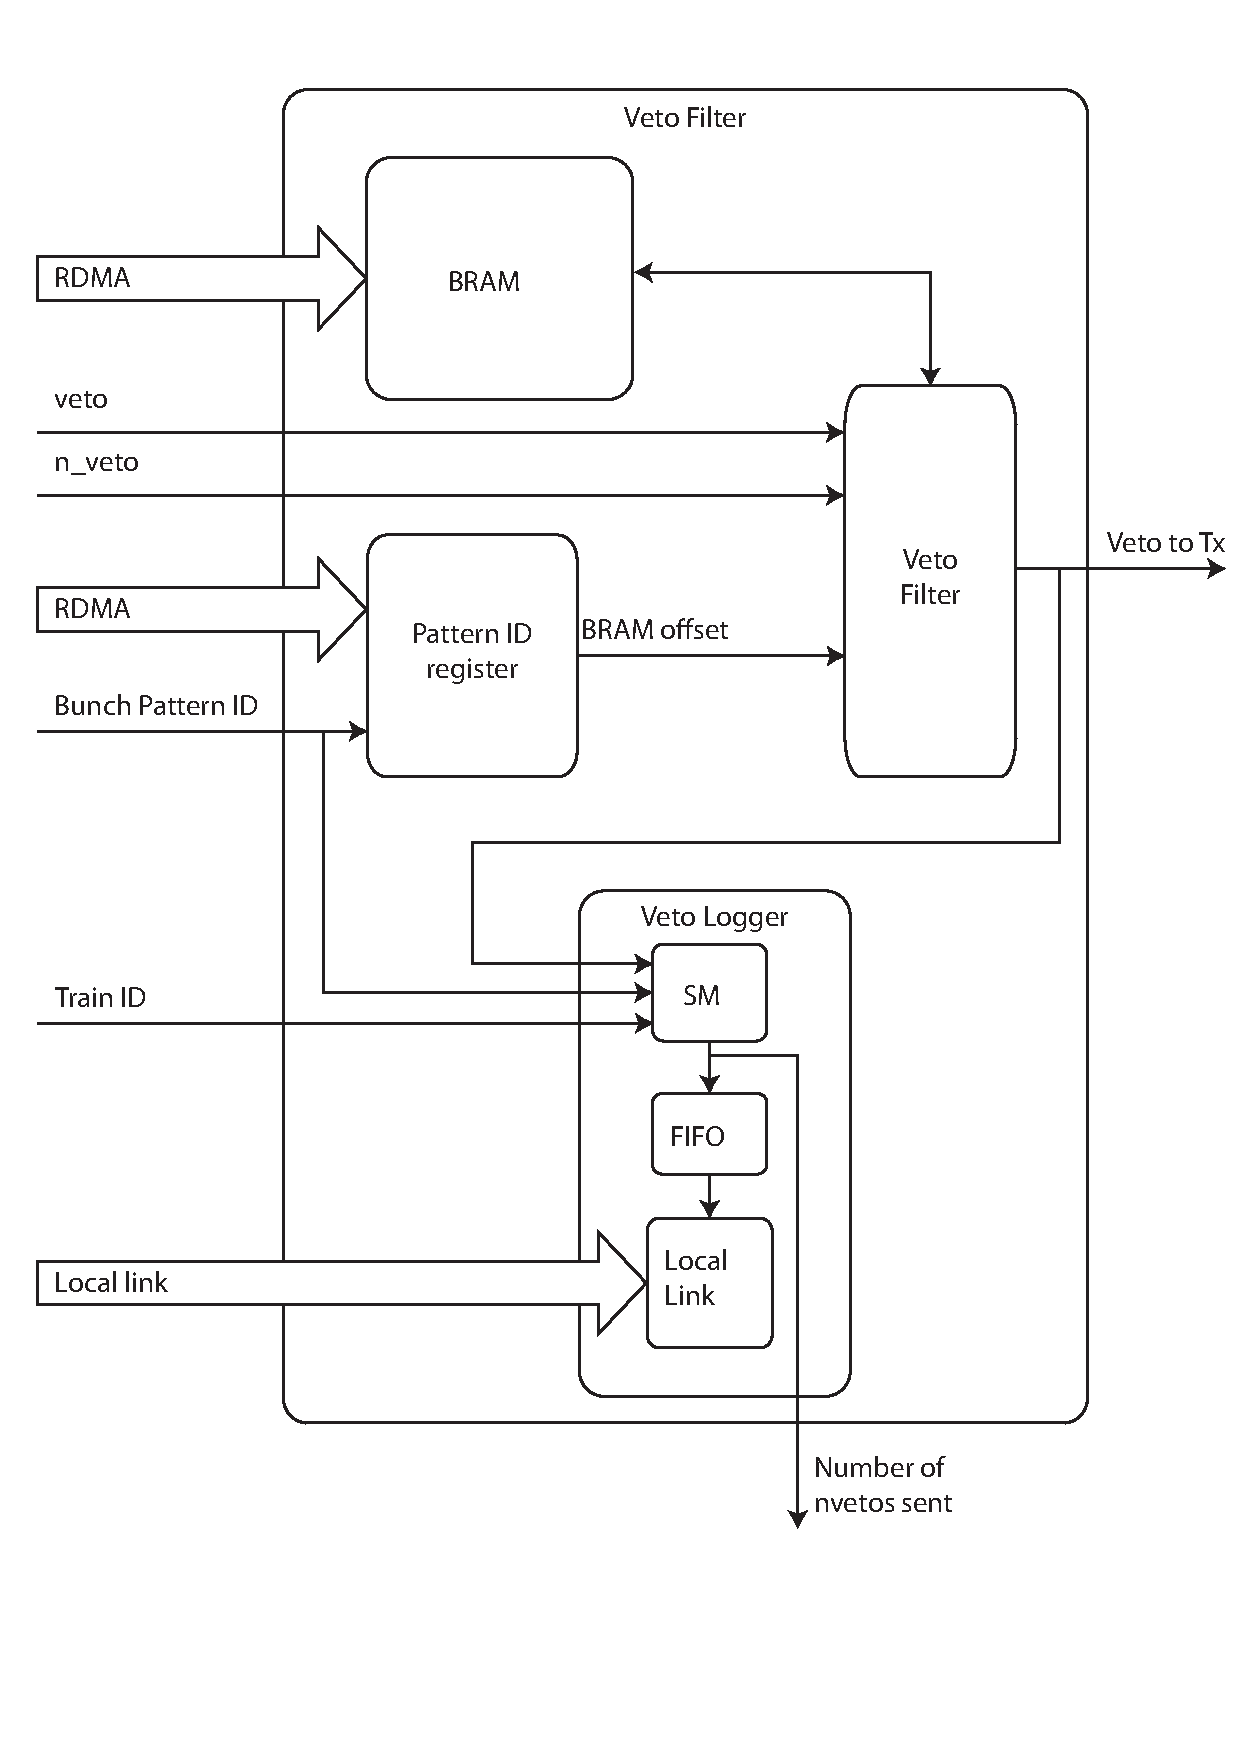
\includegraphics[width=\textwidth]{images/pdfs/veto_filter_block.pdf}
    \caption{Block diagram of the veto filter.}
    \label{fig:veto_filter_block}
\end{figure}
    
The  1024\( \times \)32b BRAM is used to store the veto patterns to be combined with the veto signal in order to form the veto decisions. To construct the veto decision and control access into the BRAM a state machine is implementing figure~\ref{fig:veto_filter_flow} was used. The veto decisions are made at the beginning of each word to reduce latency whilst BRAM and state changes are made at the end. The final block, the pattern ID register, exists to specify the mapping from bunch pattern ID to BRAM offsets.
    
\begin{figure}[htbp]
    \centering
    \includegraphics[width=\textwidth]{images/pdfs/veto_filter_flow.pdf}
    \caption{Flow diagram of the veto filter.}
    \label{fig:veto_filter_flow}
\end{figure}
    
The logging is performed using a simple state machine to feed in words to a 32b in, 256b out FIFO, this state machine (figure~\ref{fig:veto_logger_flow}) also constructs the LocalLink frame header. The header requires 8 cycles between \texttt{start\_i} being asserted and \texttt{veto\_start}, to be properly formed. The FIFO is a simple First Word Fall Through (FWFT) block with the optional \texttt{empty} and \texttt{almost\_empty} signals enabled. The read out of the FIFO is performed via a 256b-word localLink interface. Once either \texttt{stop\_i} is asserted or \texttt{N\_BUNCHES} have been counted any remaining bits of the 256b word are filled with 1's and the LocalLink's \texttt{src\_rdy} is asserted. 
    
The LocalLink interface is implemented by wrapping the FIFO's 256b \texttt{data\_out} port in some simple logic to make it conform to the local link standard. This mainly involves using \texttt{empty} to monitor the state of the FIFO, \texttt{almost\_empty} as \texttt{eof} and an internal flag from the logging state-machine for the \texttt{sof}. The \texttt{sop} (start-of-payload) signal is not used to differentiate the header from the payload as the entire frame will ultimately form part of the meta-data in the header of the read-out.
    
\begin{figure}[htbp]
    \centering
    \includegraphics[width=\textwidth]{images/pdfs/veto_logger_flow.pdf}
    \caption{Flow diagram for the veto decision logger.}
    \label{fig:veto_logger_flow}
\end{figure}

% subsection veto_implementation (end)
% section veto_filter (end)
%%%%%%%%%%%%%%%%%%%%%%%%%%%%%%%%%%%%%%%%%%%%%%%%%%%
\chapter{Transmitter} % (fold)
\label{cha:transmitter}
The transmitter block's main task is to act as the interpreter for the signals received from the CCC, translating them into command sequences that the ASIC can understand and act upon. As has been discussed above there are 4 signals that need to be translated for the ASIC: START, STOP, RESET and N/VETO. The 3 command signals all require an arbitrary number of words be sent to the ASIC whilst the veto signals are responded to by one of two words\footnote{According to the LPD manual~\cite{lpd_manual} these are `NOP' for vetos and `TRIGGER\_FLAG\_SET' for no-vetos}.
    
The transmitter can run in one of two mode: `dynamic veto mode' and `reset mode'. Dynamic veto mode is intended to be the normal mode of operation for XFEL whilst reset mode is intended for static runs with simple veto patterns (e.g. for testing). A comparison of the two can be seen in table~\ref{tab:dynamic_vs_reset_mode}. Reset mode is enabled by strobing bit 0 of the main control register (see section~\ref{sub:ctrl_reg} for details). The transmitter also has an optional minor mode called `down-scaler mode' this is primarily for versions of the ASIC that require a much slower clock during readout. When enabled it uses a multiplier (set by generic) to slow slow the clock, after a set number of cycles normal speed is resumed. 
    
\begin{table}
    \begin{center}
        % \begin{tabular}{c | p{2cm} | p{2cm}}
        \begin{tabular}{r | X{2.5cm} | X{2.5cm} }
            & \multicolumn{2}{c}{Mode} \\
            & Dynamic-veto & Reset \\
            \hline
            Standalone operation   & \xmark & \cmark \\
            Dynamic veto decisions & \cmark & \xmark \\
            \multirow{4}{*}{Signal response}
            & START  & \multirow{4}{*}{Register flag} \\
            & STOP   & \\
            & RESET  & \\
            & N/VETO & \\
        \end{tabular}
    \end{center}
    \caption{Comparison of dynamic veto and reset modes}
    \label{tab:dynamic_vs_reset_mode}
    \end{table} 
    
    \section{Interface} % (fold)
    \label{sub:tx_interface}
    The transmitter has 3 `sets' of generics: the control register reset values, the flag words (ending in \texttt{\_SIG}) and the down-scaler factor. The register resets set the default value to be written to the assorted registers if \texttt{rst} is asserted. The flag words specify certain command words that the transmitter should scan for in order to flag them for use elsewhere. The \texttt{\texttt{SYNC\_RESET}} flag is intended for use with any blocks (e.g.\ the slow command line) that have to be synchronised to the ASIC's bunch clock. The \texttt{READOUT} is intended for use by the data-receiver in order to prepare for read-out. The \texttt{DOWNSCALER\_SIG} is used to begin either the internal (if it's enabled) or an external down-scaler clock. The \texttt{DOWNSCALER\_STOP\_SIG} is only for use by an external source (the internal version counts cycles). The \texttt{DOWNSCALER\_FACTOR} specifies the factor to use for the internal down-scaler e.g.\ a factor of 100 means a scale of 100 fast clock cycles to each actual clock cycle.
    
    The in ports to the transmitter are all flags from the receiver; with the standard exception of \texttt{rst} which is the FEE internal signal (cf.\ \texttt{reset} which is the flag from the receiver).
    
    The out ports fall into 3 categories: signals to the ASIC (\texttt{ASIC\_in} and \texttt{clk\_in}), flags (marked \texttt{\_sent}) and \texttt{start\_nwords\_o}. The ASIC commands are defined in the specification. The flags have been discussed above with regards to their generic-defined trigger words. The final out port is a wrapper to the value of the \emph{start\_nwords} register (see section~\ref{sub:tx_registers}) which is used in setting the delay for \texttt{veto\_start}.
    
    The two RDMA interfaces are used for access to the command sequence BRAM and the control registers (sections~\ref{sub:tx_bram} and \ref{sub:tx_registers} respectively).
    
    \begin{table}
        \begin{center}
            \begin{tabulary}{\textwidth}{l | c | c | L}
                Name & Direction & Type & Description \\
                \hline
                REG\_RESET\_(9:0)       & & std\_logic\_vector (31:0) &  Register resets (0-9), see section~\ref{sub:tx_registers}. \\
                % TODO Add a dedicated section for signal flags? 
                \texttt{SYNC\_RESET}\_SIG            & & std\_logic\_vector (31:0) & Flag that the \texttt{SYNC\_RESET} command has been sent.                 \\
                READOUT\_SIG          & & std\_logic\_vector (31:0) & Flag that the \texttt{READOUT} command has been sent.               \\
                DOWNSCALE\_SIG        & & std\_logic\_vector (31:0) & Flag to start the down-scaler (either internal or external).\\
                DOWNSCALER\_STOP\_SIG & & std\_logic\_vector (31:0) & Flag to stop the down-scaler.                               \\
                DOWNSCALE\_FACTOR     & \multirow{-16}{*}[11.5pt]{Generic} % Avoids extra newline at top
                & integer                   & Factor for the internal down-scaler, default: 100.          \\
                \hline
                clk   & \multirow{6}{*}{in} 
                & std\_logic & The CCC clock.          \\
                rst   &  & std\_logic & FEE reset.              \\
                start &  & std\_logic & From the receiver block.\\
                stop  &  & std\_logic & \dittostraight          \\
                reset &  & std\_logic & \dittostraight          \\
                veto  &  & std\_logic & From the veto filter.   \\
                \hline
                ASIC\_in                & \multirow{7}{*}[-28.75pt]{out}
                & std\_logic                & Fast serial commands to the ASIC.  \\
                clk\_in                 &  & std\_logic                & Clock to the ASIC.  \\
                readout\_sent           &  & std\_logic                & Readout flag (for ASIC receiver block).  \\
                rsync\_sent             &  & std\_logic                & \texttt{SYNC\_RESET} flag (for slow control block).  \\
                downscaler\_start\_sent &  & std\_logic                & Downscaler start flag.  \\
                downscaler\_stop\_sent  &  & std\_logic                & Downscaler stop flag.  \\
                start\_nwords\_o        &  & std\_logic\_vector (31:0) & Number of words used for `START' to set veto\_start delay.\\
                \hline
                bram\_rdma & \multirow{2}{*}[-17.25pt]{Interface} 
                & RDMA & Interface to the ASIC command word BRAM. Mask: 0x000003FF. \\
                ctrl\_rdma & & RDMA & Interface to the control register. Mask: 0x0000000F. \\
            \end{tabulary}
        \end{center}
        \caption{Interface for the transmitter block}
        \label{tab:tx_interface}
    \end{table}
  
    % subsection tx_interface (end)
    \section{Registers} % (fold)
    \label{sub:tx_registers}
    There are two externally accesible sets of registers in the transmitter block, a control register and the command BRAM both are accessed via RDMA (see appendix~\ref{cha:rdma_interface}). The control registers direct the flow of the state machine whilst the BRAM stores the instruction sets to be sent to the ASIC. There are 3 commands that the block has instruction sets for: START, STOP and RESET. Obviously these are normally received via the receiver module but the RESET command can also be sent using a toggle in the control register.
    \subsection{Control register} % (fold)
    \label{sub:ctrl_reg}
    The control register specifies 10 registers:
    \begin{description}
        \item[1] The general state-machine control register that toggles various modes (i.e. whether to use the down-scaler module and manual RESET) as well as how many bits to send downscaled if that mode is enabled.
        \item[2-7] 3 pairs of registers that store the number of words (shortened to `nw') and offsets for the 3 different instruction sets (i.e. one \emph{-nw} and one \emph{-offset} for each of START, STOP and RESET).
        \item[8] The word to be sent in case of a veto.
        \item[9] The word to be sent in case of a no-veto.
        \item[10] The status register, indicates what state the statemachine is in.
    \end{description}
    default values and addresses are given in table~\ref{tab:ctrl_reg_default}.
    
    The state-machine control register takes values of the following format:
    \begin{align} \label{fmt:control_reg}
        <\text{DOWNSCALER\_ENABLE } 32>\ldots<\text{DOWNSCALER\_BITS } 20:5>\ldots<\text{RESET\_MODE\_EN } 0>
    \end{align}
    `RESET\_MODE\_EN' is a flag to manually start the state-machine in reset mode i.e. reset\_nwords worth of commands from reset\_offset in the BRAM will be sent. This mode can be used instead of dynamically determining the veto to be sent in a `fire and forget' manner.

    `DOWNSCALER\_ENABLE' indicates that the internal down-scaler should be used to send the next `DOWNSCALER\_BITS', this means that the maximum number of bits that can be sent at the down-scaled rate is \(2^{16} - 1\), i.e. 65,536 or 2,978\(\times\)22b words. Obviously if down-scaling is being handled by an external clock this restriction doesn't apply.

    The BRAM offsets and command sequence lengths (\emph{-offset} and \emph{-nw} registers respectively) have maximum values determined by the size of the BRAM i.e.\ 1,024. These values are set using the LSB of the word i.e.\ 9 down-to 0. Obviously setting an \emph{-offset} to 1,024 will result in only 1 word and unless the corresponding \emph{-nw} is set to 1 this will result in an address overflow and undefined behaviour. By the same token setting an \emph{-nw} register to 1,024 is allowed but will mean that any other commands to be sent must be either specified as subsets of this command sequence or not used.\footnote{This could be useful if using the reset-mode or in dynamic mode if \texttt{RESET} is not expected to be used.}
    
    The veto/nveto\_word registers specify the appropriate words to send when in dynamic-veto mode, the defaults are \texttt{NOP} and \texttt{TRIGGER\_FLAG\_SET} respectively. When run in this way the state-machine progresses START\(\rightarrow\)vetoes\(\rightarrow\)STOP with vetoes being determined by the veto filter.
      
    The status register is a read only register that logs which state the state-machine is in and has the following format:
    \begin{align} \label{fmt:status_reg}
        <\text{state\_machine\_enabled } 31>\ldots<\text{RESET } 3> <\text{STOP } 2> <\text{DYNAMIC\_VETO } 1> <\text{START } 0>
    \end{align}
	  
    \begin{table}
        \begin{center}
            \begin{tabular}{c|c | c |c}
                Address & Description             & Reset generic      & Default value  \\
                \hline                    
                0x1     & SM-Control              & CTRL\_REG\_RESET   & 0x00000000     \\ 
                0x2     & Start: offset           & START\_OFF\_RESET  & 0x00000000     \\  
                0x3     & Start: number of words  & START\_NW\_RESET   & 0x00000006     \\ 
                0x4     & Stop: offset            & STOP\_OFF\_RESET   & 0x00000006     \\ 
                0x5     & Stop: number of words   & STOP\_NW\_RESET    & 0x00000007     \\ 
                0x6     & Reset: offset           & RESET\_OFF\_RESET  & 0x0000000D     \\ 
                0x7     & Reset: number of words  & RESET\_NW\_RESET   & 0x0000000F     \\ 
                0x8     & Veto word               & VETO\_WORD\_RESET  & 0x00210000     \\ 
                0x9     & No-veto word            & NVETO\_WORD\_RESET & 0x00200000     \\ 
                0xA     & Status                  & n/a                & 0x00000000     \\ 
            \end{tabular}
        \end{center}
        \caption{Control register layout. With the exception of the status register the reset values of each register can be changed by setting the appropriate reset-generic, these values only take affect when the `rst' line is asserted \textbf{not} when the RESET signal is received.}
        \label{tab:ctrl_reg_default}
    \end{table}

    % subsubsection control_regsiter (end)
    \subsection{Instruction set BRAM} % (fold)
    \label{sub:tx_bram}
    The BRAM used to store the instruction sets is 1024\(\times\)32b words. The ASIC expects 20b commands of the format:
    \begin{align}\label{fmt:asic_format}
        <\text{SYNC }19><\text{X }18<\text{CMD } 17:10><\text{PADDING\_ZEROS } 9:0>
    \end{align}
    if a word length greater than 20b is being used (e.g. 22b, the current default) then the zero-padding is extended as required. The `SYNC' bit is a `1' and `X', by convention, a `0' these are automatically prepended by the state machine. The only exception to this is the 20b command \texttt{SYNC\_RESET} (currently set to be 0x5A5A5) which overrides the above format.

    Words not defined by the ASIC are ignored so internal flag triggers (e.g. for `DOWNSCALER\_START') need not be defined ASIC commands.

    The BRAM expects words to have the format:
    \begin{align}\label{fmt:tx_bram}
        <\text{N\_NOPS } 31:\text{WORD\_LENGTH }><\text{COMMAND } (\text{WORD\_LENGTH} - 1):0>
    \end{align}
    The COMMAND is expected to be correctly padded e.g. if 22b words are being used for a normal command the last 12b should be `0'. The SYNC bit doesn't need to be set. N\_NOPS indicates how many \texttt{NOP} commands should follow the COMMAND, a NOP is pre-defined to be a SYNC-bit followed by the appropriate number of 0's. It is important to note that NOPs contribute to the number of words sent for any state and a NOP sent as a member of N\_NOPS must not be the final command

    \textbf{Example:} if, for the \texttt{START}-sequence and using 22b words, \texttt{POWER\_UP} (0x02\footnote{see table~\ref{tab:asic_command_words}}) followed by 4 NOPS is to be sent then the first two locations in BRAM could be set to `0x00C08000' and `0x00000000'. 0x00C specifies 3 NOPS (\(\text{0xC}<<2 = 0x3\)\footnote{Where `\(<<\)' is a left-shift, the \( <<2 \) is account for the 2~MSB of the command.}) and 0x08000 is the command (\(\text(0x02) << 22 \)) with the appropriate padding. The final entry of 0x00000000 is the 4\(^{\text{th}}\) NOP; its SYNC bit will be automatically set.
    % subsubsection tx_bram (end)
    % subsection tx_registers (end)
    \section{Implementation} % (fold)
    \label{sub:tx_implementation}
    
    The transmitter block has 3 key responsibilities:
    \begin{itemize*}
        \item To transmit preset \texttt{START}/\texttt{STOP}/\texttt{RESET} command sequences. 
        \item To transmit either the \texttt{VETO} or \texttt{NO-VETO} word for each bunch, at run-time, as determined by the veto filter.
        \item Maintain a constant latency with respect to the bunch clock. 
    \end{itemize*}
    There are also several ancillary requirements:
    \begin{itemize}
        \item Provide information to other blocks on the command stream being sent to the ASIC (e.g. if the command \texttt{SYNC\_RESET} is sent).
        \item Provide a mechanism to slow the clock sent to the ASIC for read-out (only required for ASIC~v1).
        \item Allow reconfiguration of the command sequences.
        \item Ensure proper setting of synchronisation bits.
    \end{itemize}
    
    To meet the above requirements two processes were implemented: the shift-block to serialise and inspect command sequences; and the state-machine that determines when to change state and which command sequences to use. Previously, these responsibilities were split across multiple blocks but to simplify state sharing and meet the latency requirements they were merged into a single block. Figure~\ref{fig:tx_block} shows a block diagram of the transmitter, both the shift-block and state-machine are within the state-machine block.
    
    \begin{figure}[htbp]
        \centering
        \includegraphics[width=\textwidth]{images/pdfs/tx_block.pdf}
        \caption{Block diagram of the transmitter.}
        \label{fig:tx_block}
    \end{figure}
        
    The shift-block primarily acts as a shift register to serialise the command words being sent to the ASIC. It has two secondary functions that require inspection of the commands being serialised: flagging and setting sync-bits. Some of the other components of the firmware require certain command words be flagged for their own functionality (e.g. the slow command needs to know when \texttt{SYNC\_RESET} is sent). To do this when a word is loaded from the BRAM (and only from the BRAM) it is compared to the 4 pre-set words given in table~\ref{tab:shift_block_flags}, if it matches one then the appropriate flag is set. These words are tested sequentially, in the order given in the table, so if a word matches multiple triggers only the flag corresponding to the first match will be set. The flag words are set via generics and are not expected to change, flags do not have to be valid ASIC words although the ASIC's response to unknown commands is undefined and should be confirmed prior to use. At the same time as checking for flags the first two bits of each word are set appropriately: for \texttt{SYNC\_RESET} they are set to `01' and all other words `10' as specified in \cite{lpd_manual}. These sync-bits are not included in tests for flags. The shift-block's functionality for the different states are given in table~\ref{tab:shift_block_behaviour}, the different states are described below.

    \begin{table}
        \begin{center}
            \begin{tabular}{c|c|l}
                Flag             & Default    & Notes \\
                \hline
                rsync             & 0x00069694 & Used to keep the slow command line synced to the ASIC.   \\
                readout           & 0x00044400 & Used to alert the readout receiver block of input.       \\
                down-scaler start & 0x00044000 & Moving to the slower clock (either internal or external).\\
                down-scaler stop  & 0x00055000 & Stop using the slow clock (external only).               \\
            \end{tabular}
        \end{center}
        \caption{Flag information, these are command words that the shift-block looks for and will flag along. Default values are for 22b words, see section~\ref{sub:tx_bram} for more details. When looking for flags the sync bits (the first two bits) are ignored so do not need to be set.}
        \label{tab:shift_block_flags}
    \end{table}
    
    \begin{table}
        \begin{center}
            \begin{threeparttable}
                \begin{tabular}{r|c|c|l}
                    State & Flags enabled & Sync-bit set & Command source                        \\
                    \hline                                                                       
                    IDLE  &    \xmark     &    \xmark    & n/a                                   \\
                    NOPS  &    \xmark     &    \cmark    & State machine, command = 0x0\tnote{1}.\\
                    VETO  &    \xmark     &    \cmark    & State machine, either veto or no-veto.\\
                    START &    \cmark     &    \cmark    & BRAM: START command sequence.         \\
                    STOP  &    \cmark     &    \cmark    & BRAM: STOP command sequence.          \\
                    RESET &    \cmark     &    \cmark    & BRAM: RESET command sequence.         \\
                \end{tabular}
                \begin{tablenotes}
                    \scriptsize
                    \item[1] i.e. 0x200000 is the full 22b command, including sync-bit.
                \end{tablenotes}
                \caption{Description of the shift-block's behaviour depending on state.}
            \end{threeparttable}
        \end{center}
        \label{tab:shift_block_behaviour}
    \end{table}
    
    \begin{figure}[htbp]
        \centering
        \includegraphics[height=\textheight]{images/pdfs/tx_sm_flow.pdf}
        \caption{Schematic of the control flow in the transmitter block.}
        \label{fig:tx_sm_flow}
    \end{figure}
    
    The second process, the state-machine, is mainly concerned with maintaining position within each command sequence, changing state and controlling the BRAM. Figure~\ref{fig:tx_sm_flow} shows the relationship between the different states and the causes for state changes; figure~\ref{fig:tx_sm_bram_control_flow}, meanwhile, shows how access to the BRAM is determined. During state changes the source of the next word is set according to the sources in table~\ref{tab:shift_block_behaviour}, obviously this change occurs before the actual state changes. It's important to note that, as discussed in section~\ref{sub:tx_bram} the final word of any sequence should not be a NOP sent from the NOP state as control returns to the origin state, e.g. `START\( \rightarrow \)NOPS\( \rightarrow \)VETO' is not permitted. 
    
    \begin{figure}[htbp]
        \centering
        \includegraphics[scale=0.7]{images/pdfs/tx_sm_bram_control_flow.pdf}
        \caption{General control logic flow for START, STOP and RESET states.}
        \label{fig:tx_sm_bram_control_flow}
    \end{figure}
    % subsection tx_implementation (end)
    % section transmitter (end)
    %%%%%%%%%%%%%%%%%%%%%%%%%%%%%%%%%%%%%%%%%%%%%%%%%%%
    \chapter{Timing Diagrams} % (fold)
    \label{cha:timing_diagrams}
    \section{Start, no-veto, stop} % (fold)
    \label{sec:start_no_veto_stop}
    Figure~\ref{fig:isim_start-veto-stop} shows a very simple dynamic sequence with a single no-veto word being sent prior to stopping. It shows the \texttt{log\_start} which indicates that the train ID and bunch pattern ID have been received and that the veto logger should add them to the header. \texttt{veto\_start} starts the veto filter as the first veto command is received.
    \begin{figure}[htbp]
        \centering
        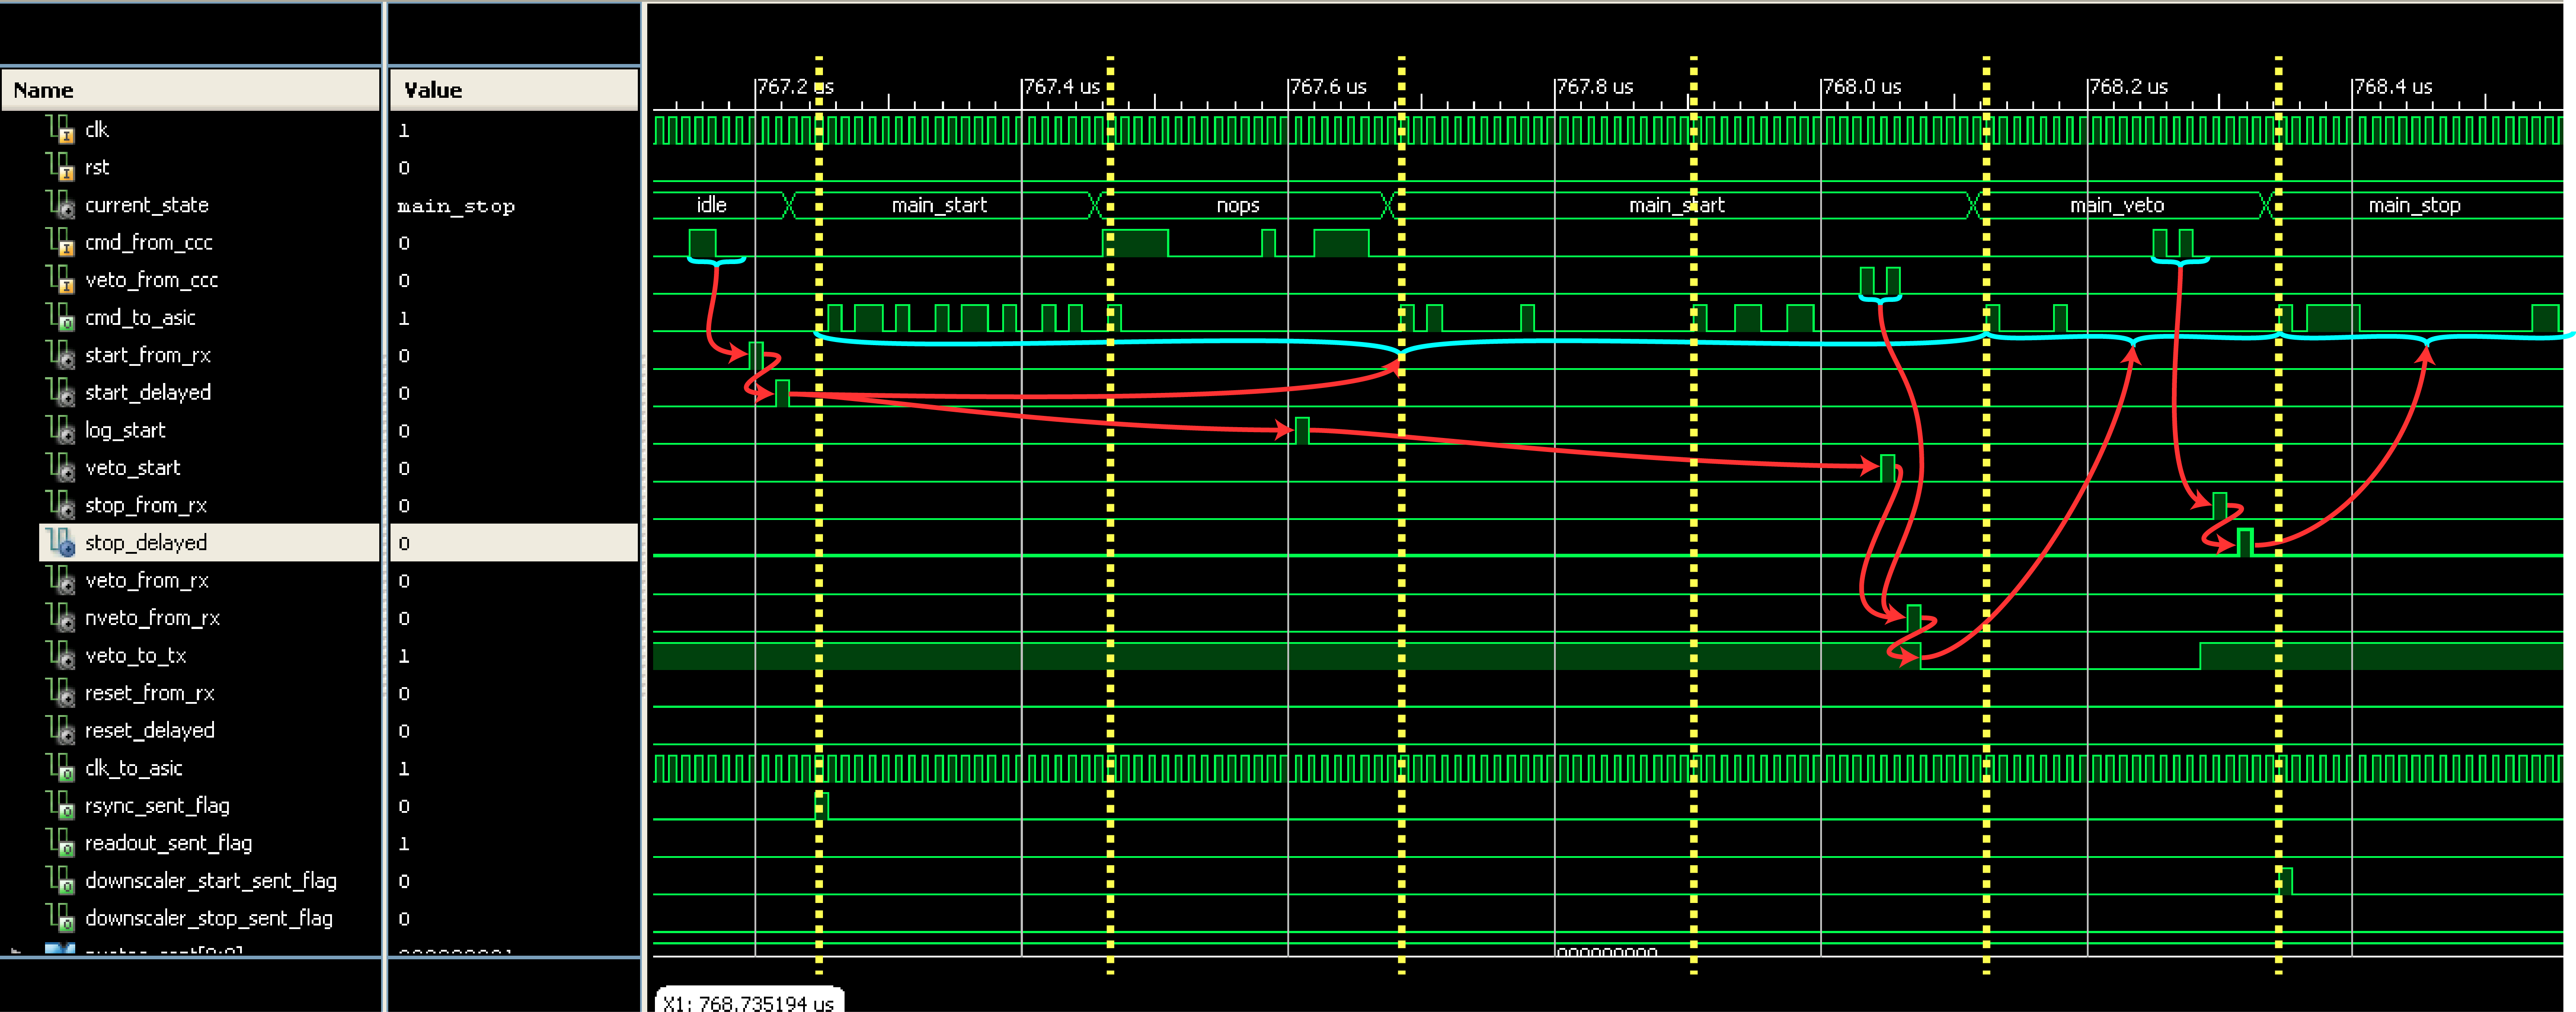
\includegraphics[width=\textwidth]{images/isim/edited/start-veto-stop.png}
        \caption{A \texttt{START}, \texttt{NO-VETO}, \texttt{STOP} sequence with a single \texttt{NO-VETO} prior to the stop signal. The blue braces indicate either input/output word sequences whilst the red lines show logical sequences.}
        \label{fig:isim_start-veto-stop}
    \end{figure}
    % section start_no_veto_stop (end)
    \section{Veto/No-veto} % (fold)
    \label{sec:veto_no_veto}
    Figure~\ref{fig:isim_veto_no_veto} shows the dynamic veto mode in operation, 3 vetoes followed by 6 no-vetoes. The \texttt{veto\_to\_tx} line shows the command received by the transmitter.
    \begin{figure}[htbp]
        \centering
        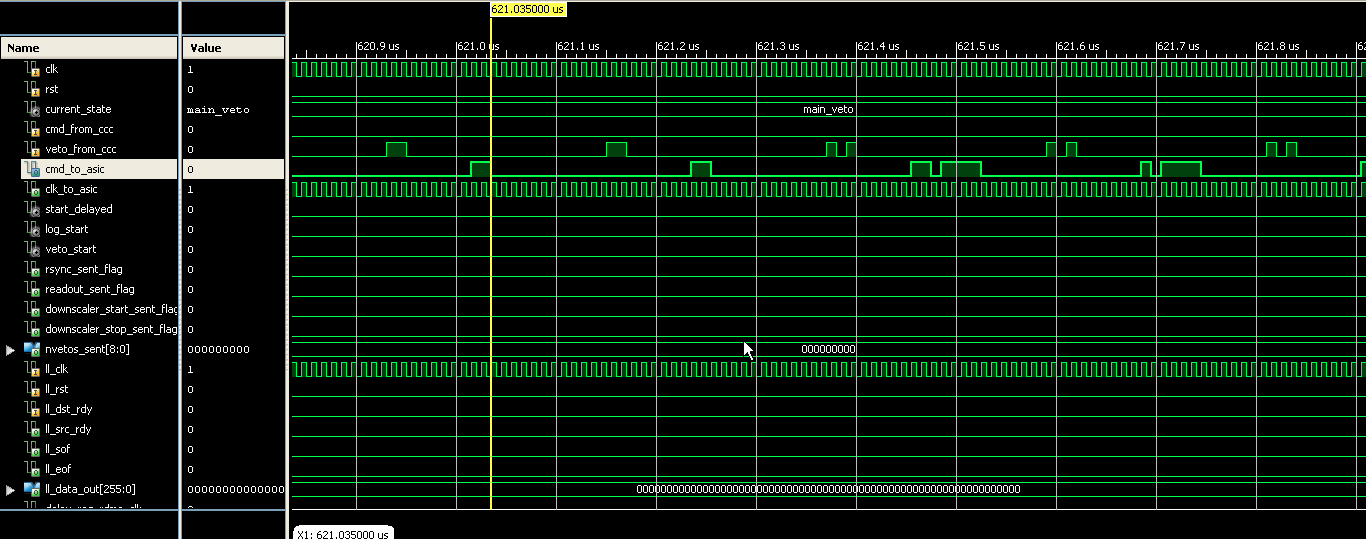
\includegraphics[width=\textwidth]{images/isim/edited/veto_no_veto.png}
        \caption{A selection of vetoes/no-vetoes.}
        \label{fig:isim_veto_no_veto}
    \end{figure}
    % section veto_no_veto (end)
    \section{Reset Command} % (fold)
    \label{sec:reset_command}
    Figure~\ref{fig:isim_reset_cmd} shows the reset sequence being sent in response to the \texttt{RESET} command from the CCC. The first word of the \texttt{RESET} command sequence is a \texttt{RSYNC} so the \texttt{rsync\_sent\_flag} is asserted. Figure~\ref{fig:isim_reset_rdma} shows the same thing being triggered via the control register (being set via RDMA).
    \begin{figure}[htbp]
        \centering
        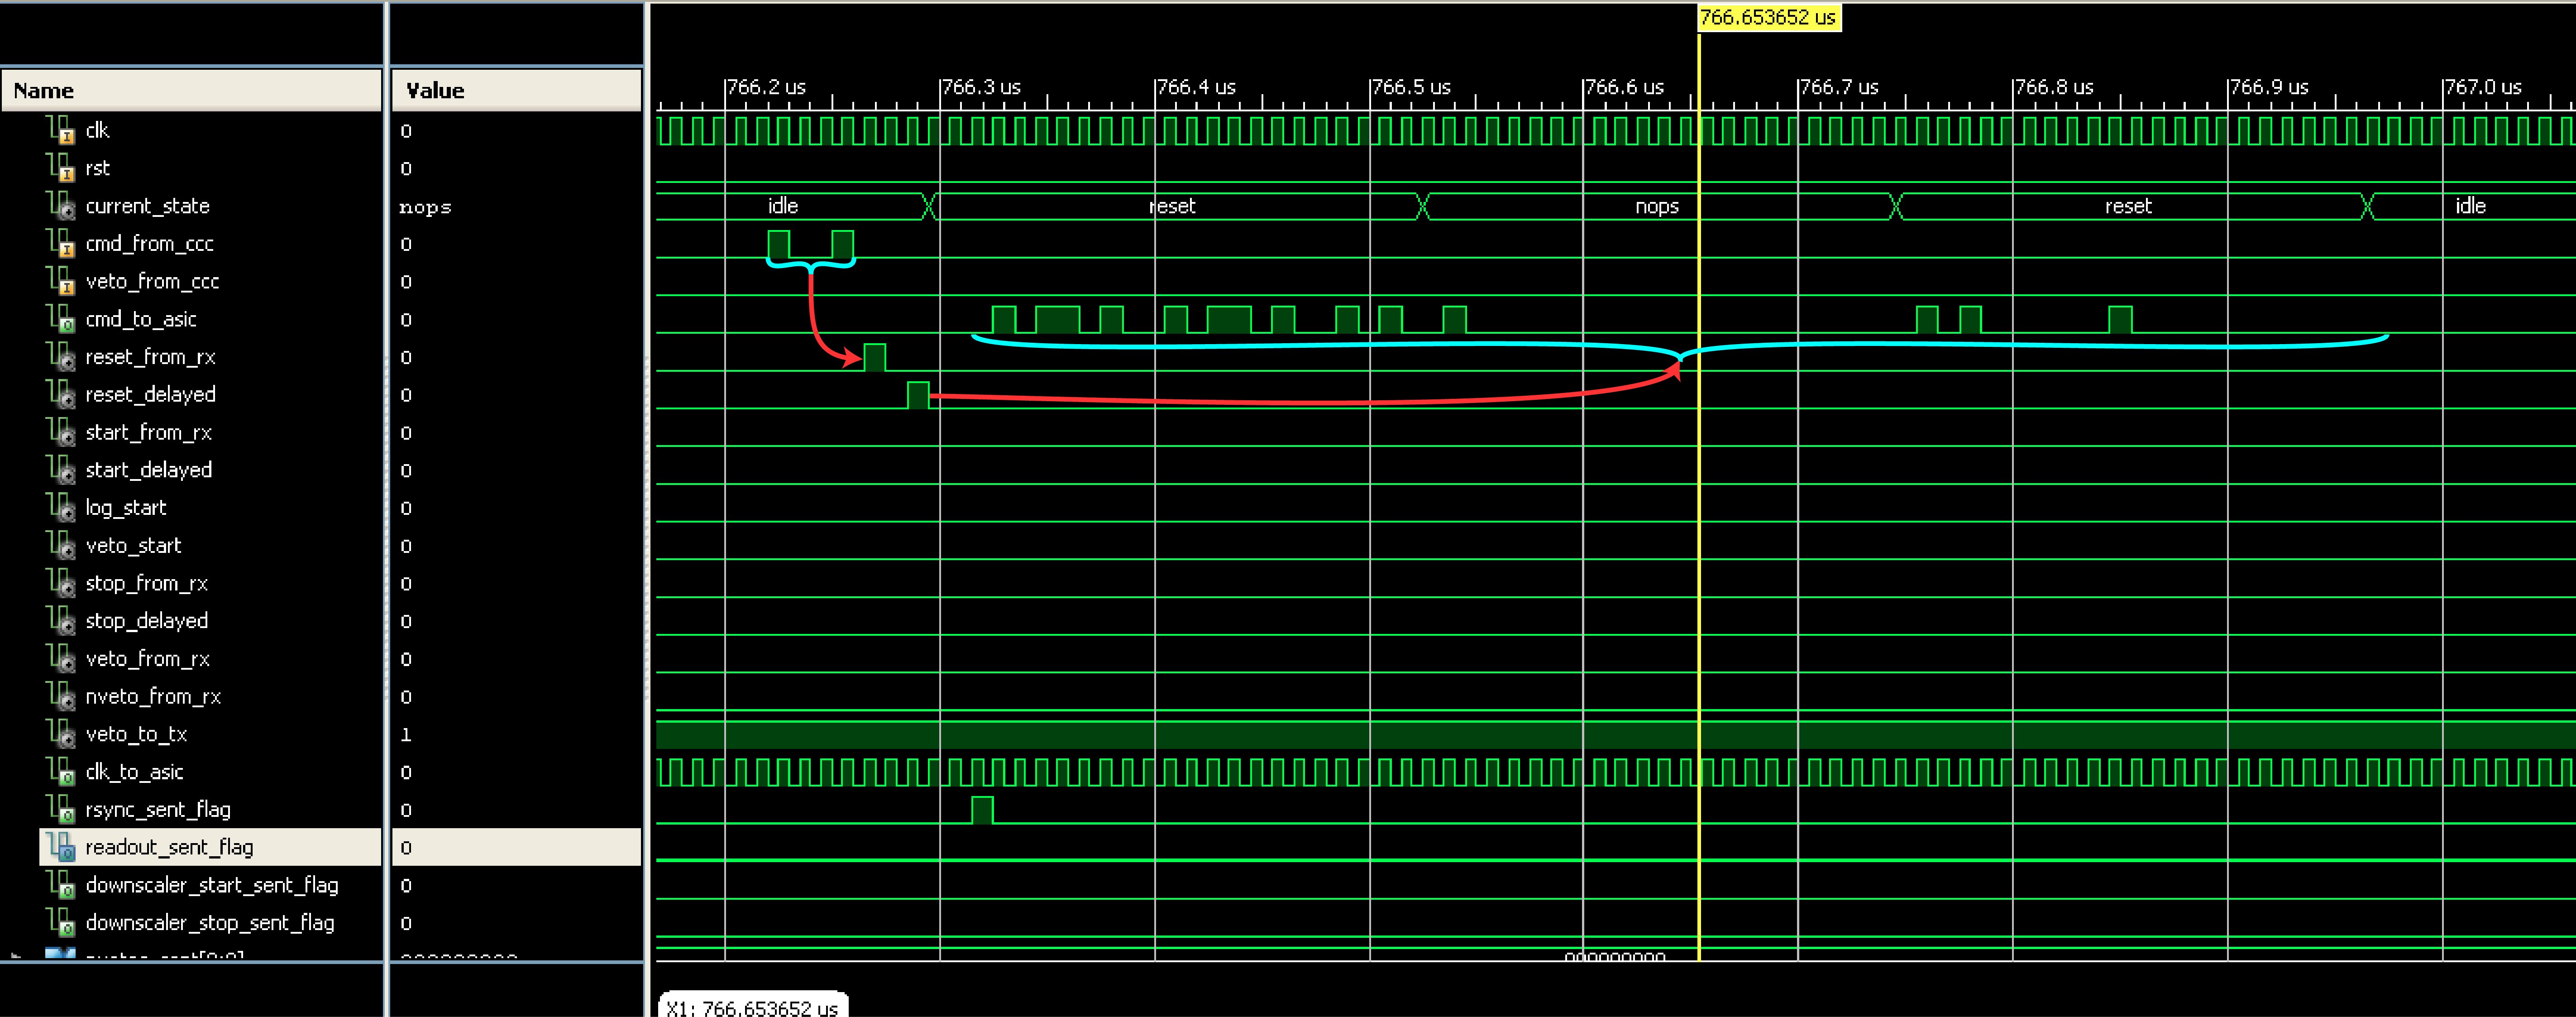
\includegraphics[width=\textwidth]{images/isim/edited/reset_cmd.png}
        \caption{The reset sequence being triggered by the cmd line from the CCC.}
        \label{fig:isim_reset_cmd}
    \end{figure}
    \begin{figure}[htbp]
        \centering
        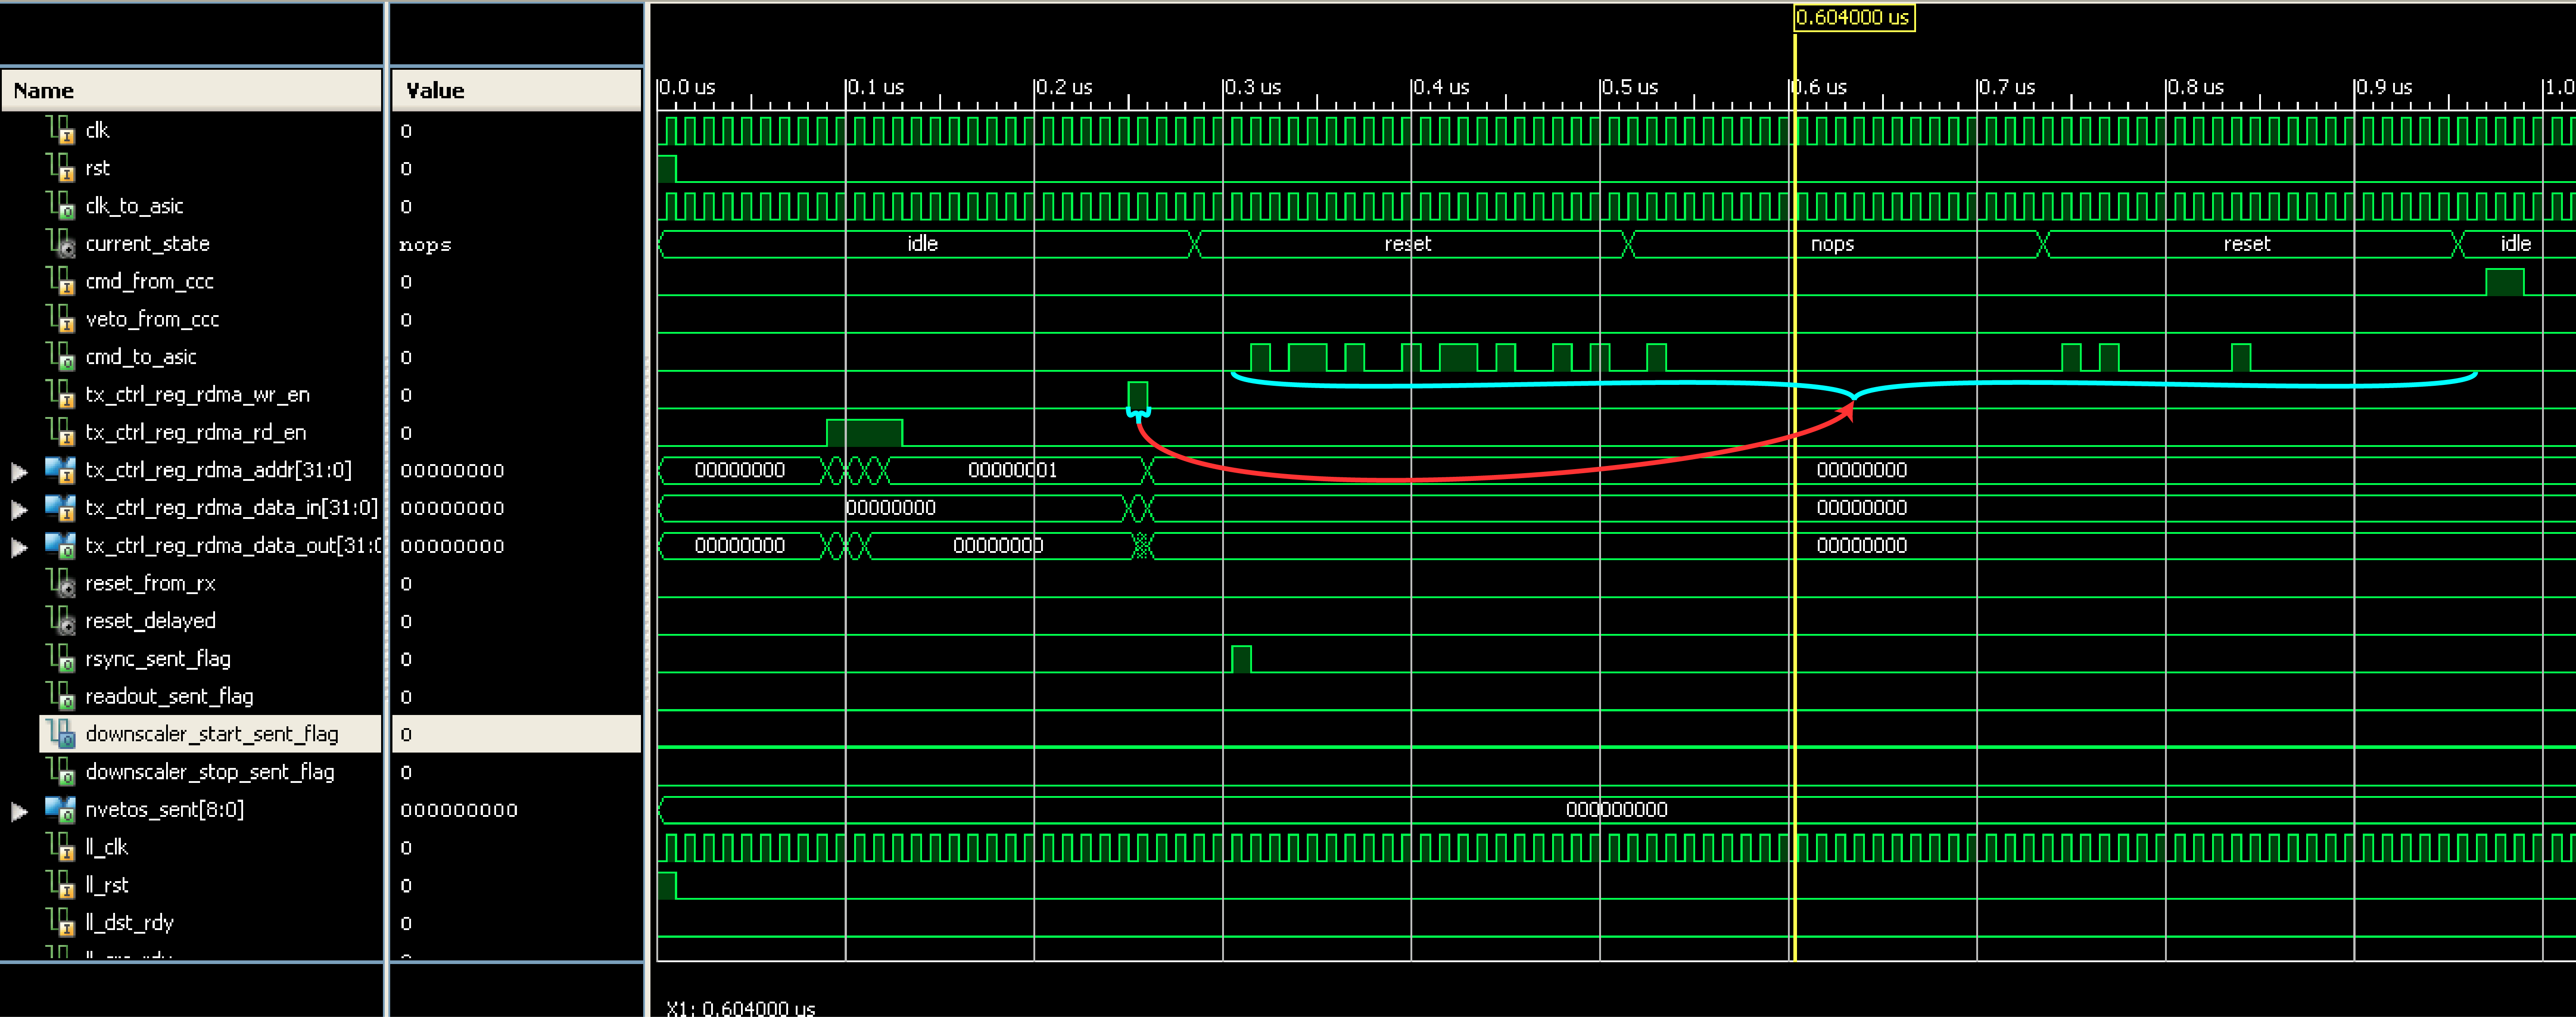
\includegraphics[width=\textwidth]{images/isim/edited/reset_rdma.png}
        \caption{The reset sequence being triggered via the control register.}
        \label{fig:isim_reset_rdma}
    \end{figure}
    % section reset_command (end)
    \section{Stop with down-scaler} % (fold)
    \label{sec:stop_downscaler}
    Figures~\ref{fig:isim_stop-downscaler}~and~\ref{fig:isim_stop-downscaler-zoom} show the stop command triggering the down-scaler.
    \begin{figure}[htbp]
        \centering
        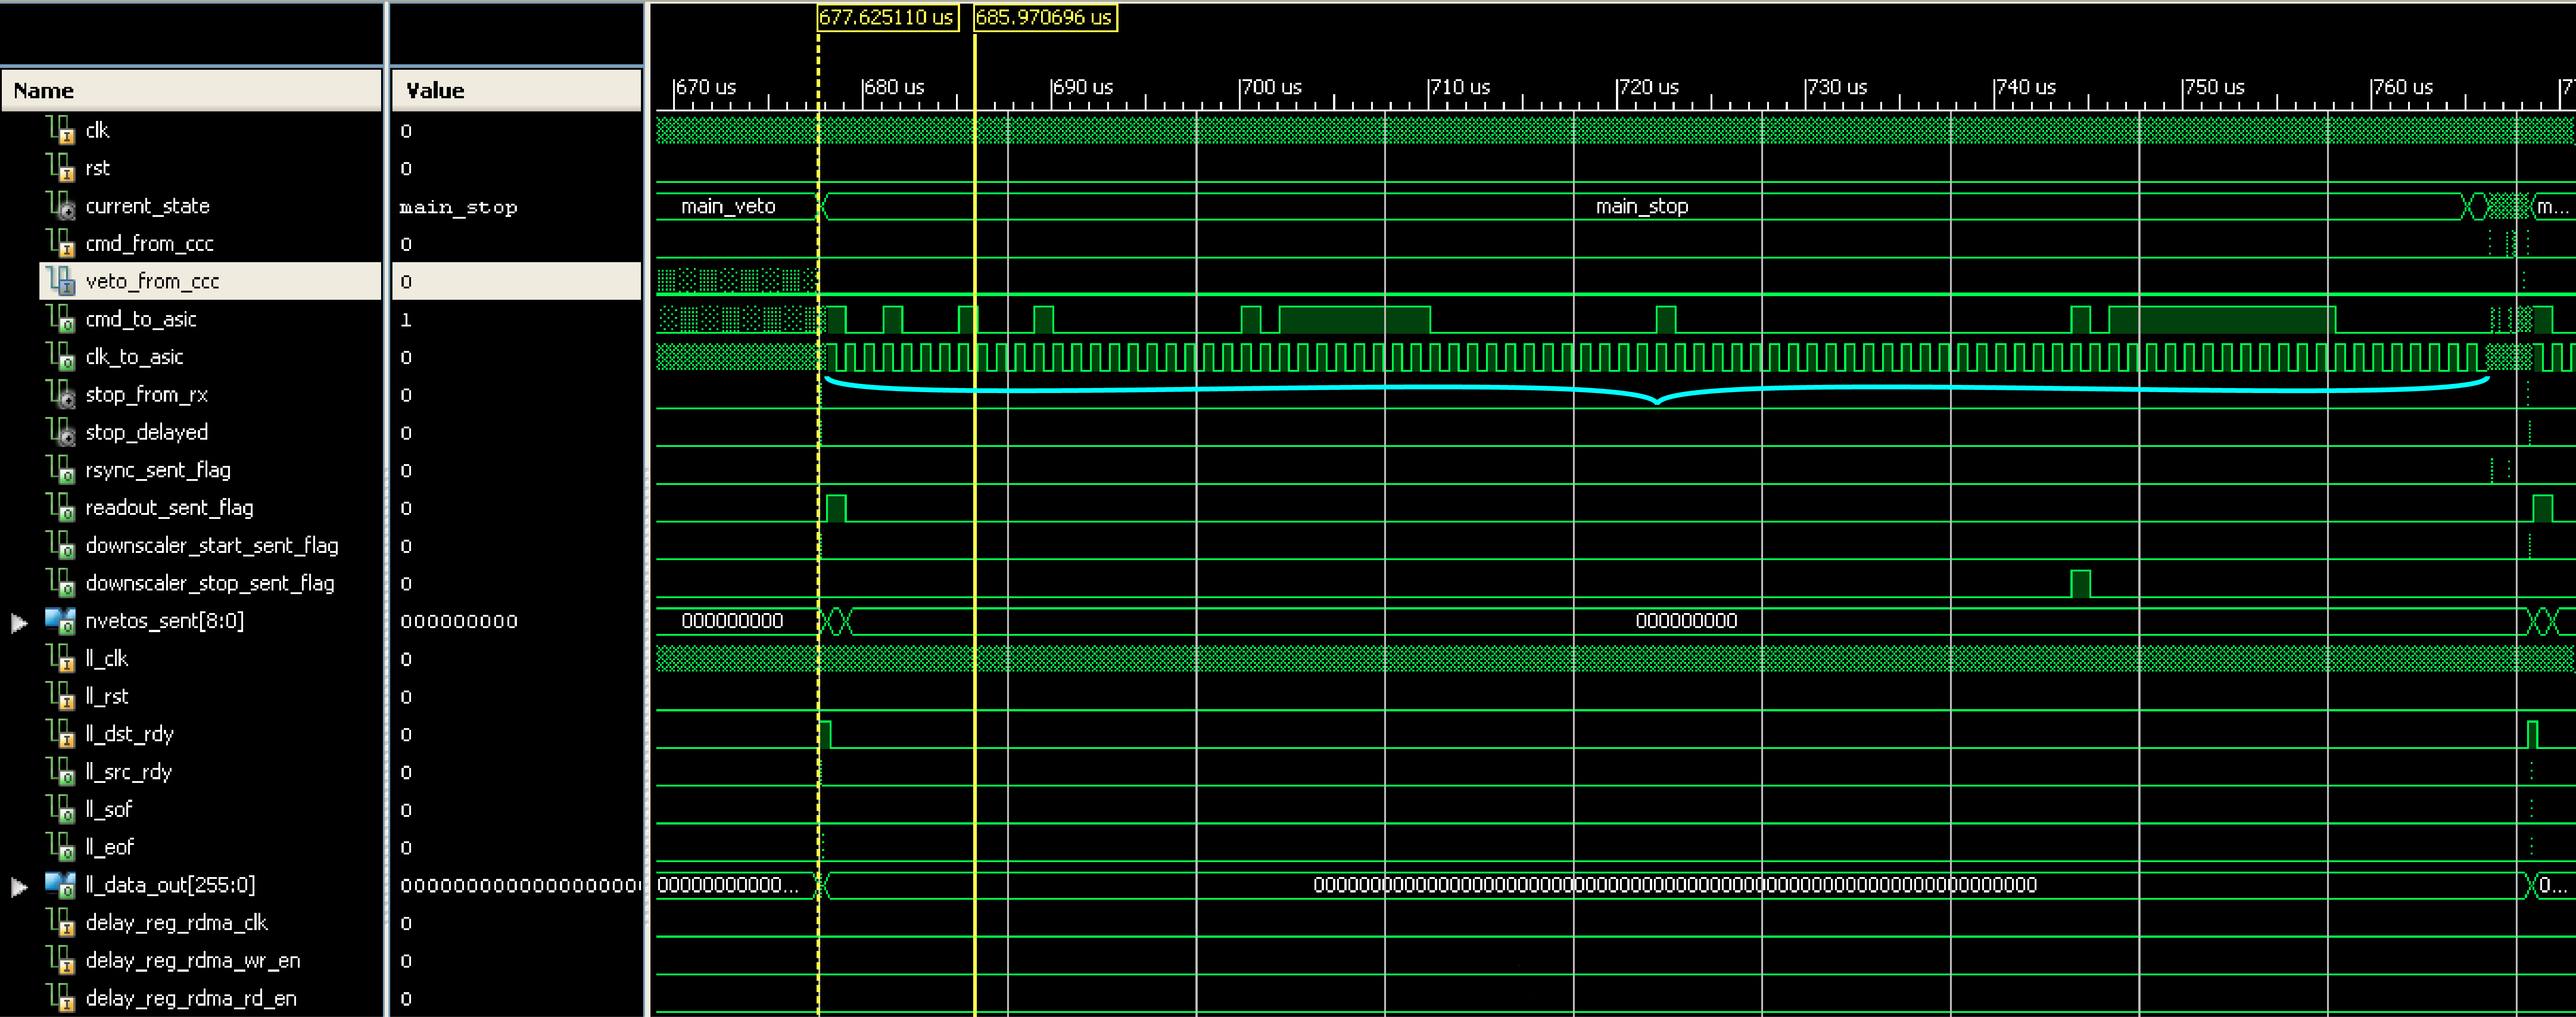
\includegraphics[width=\textwidth]{images/isim/edited/stop-downscaler.png}
        \caption{The \texttt{clk\_to\_asic} down-scaled by a factor of 100. The section delimitated by the yellow guides is shown in figure~\ref{fig:isim_stop-downscaler-zoom}. Note that the second word sent (after the down-scaler trigger) is the \texttt{READ\_OUT\_START} command, the flag is also down-scaled.}
        \label{fig:isim_stop-downscaler}
    \end{figure}
    
    \begin{figure}[htbp]
        \centering  
        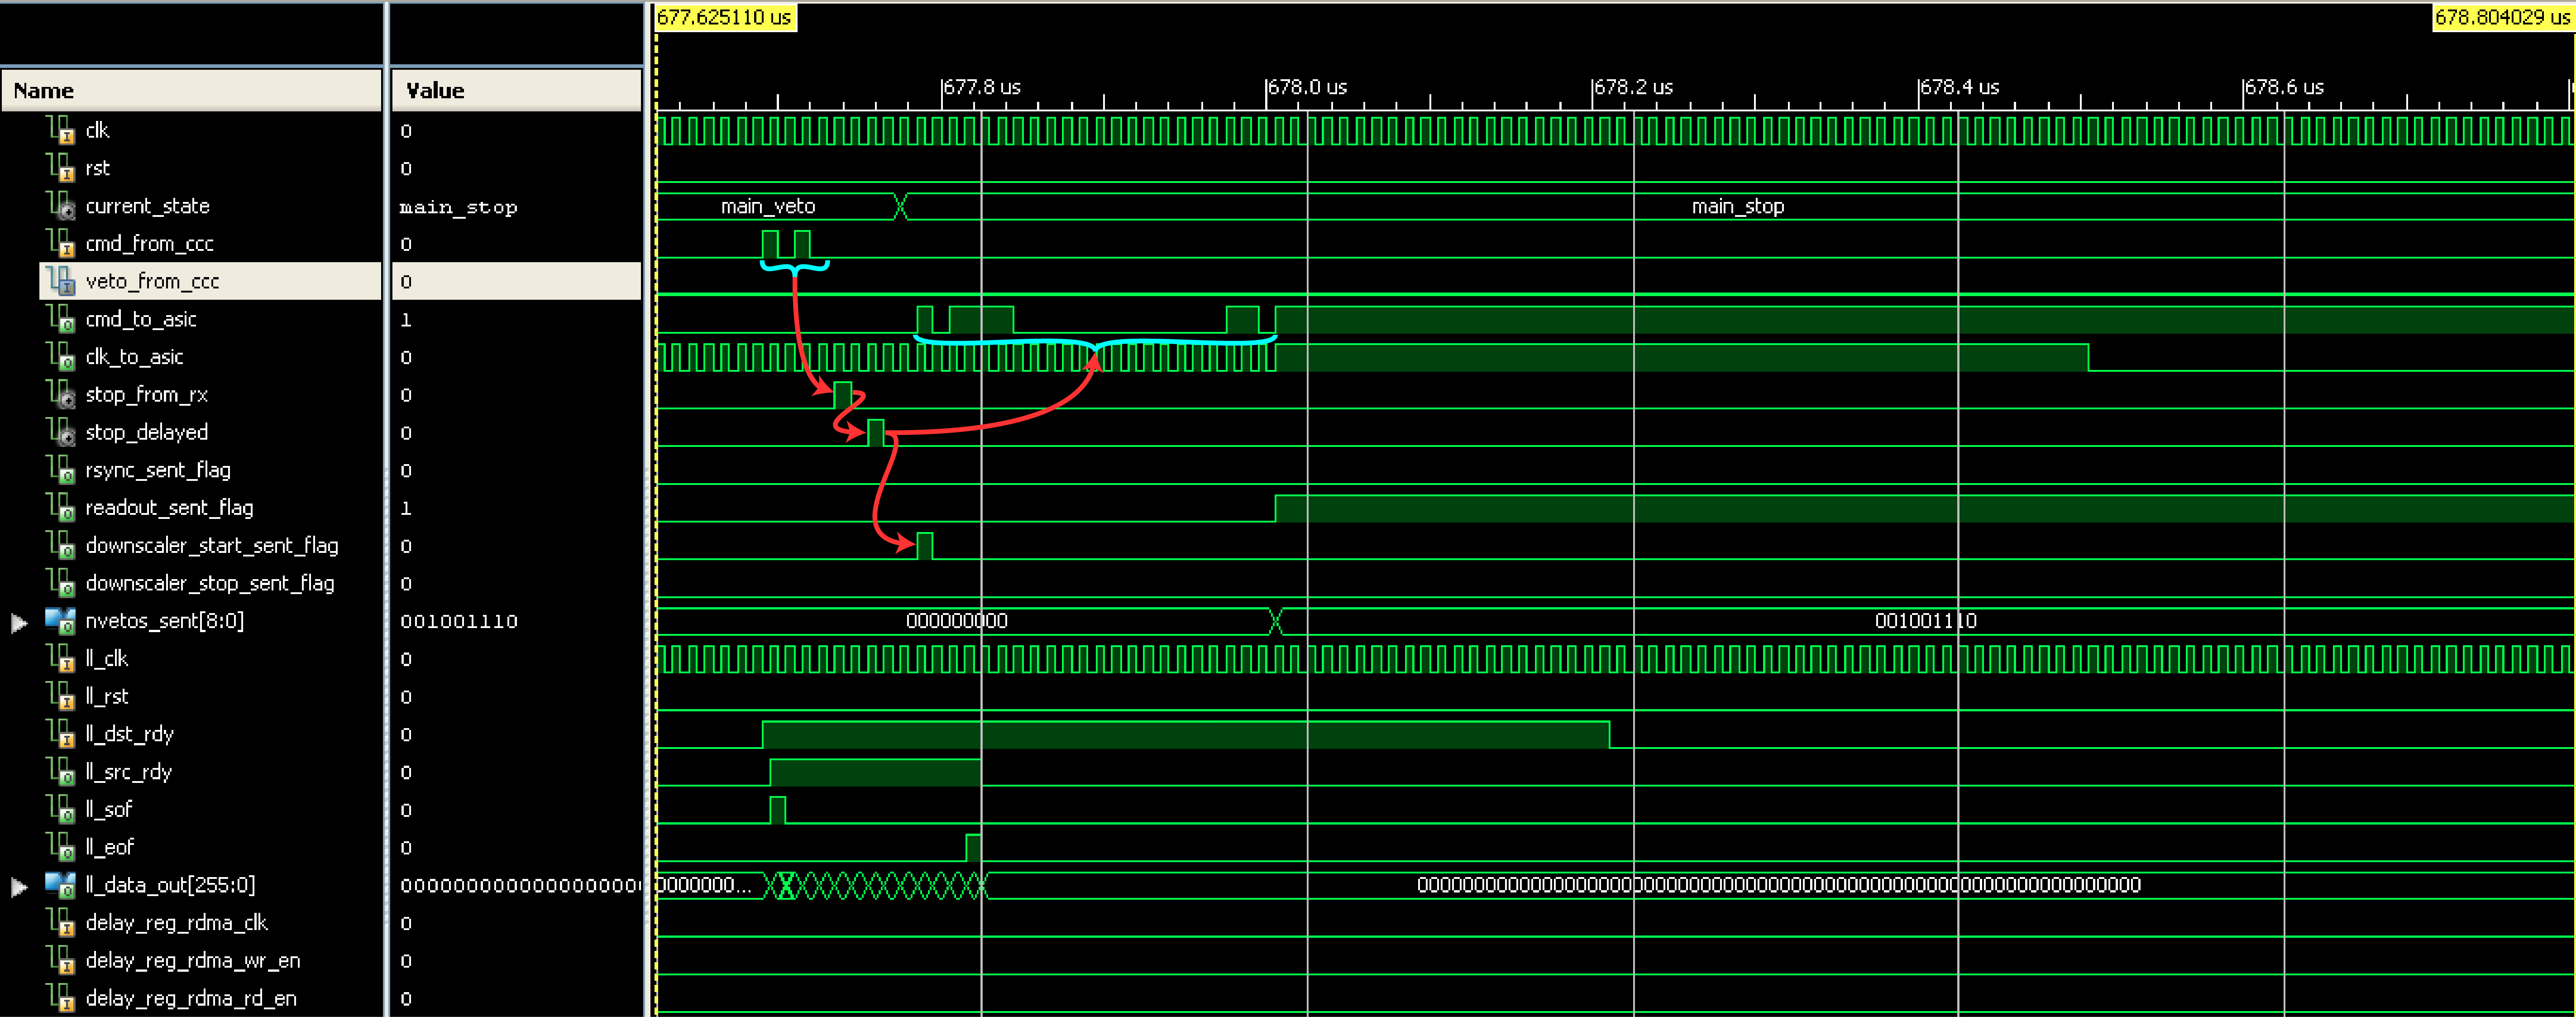
\includegraphics[width=\textwidth]{images/isim/edited/stop-downscaler-zoom.png}
        \caption{The \texttt{STOP} command and down-scaler start word being sent. }
        \label{fig:isim_stop-downscaler-zoom}
    \end{figure}
    % section stop_downscaler (end)
    \section{RDMA} % (fold)
    \label{sec:rdma}
    Figure~\ref{fig:isim_rdma} shows a simple test of the RDMA accessible registers and BRAMs. The first 4 locations in each are read out. 
    \begin{figure}[htbp]
        \centering
        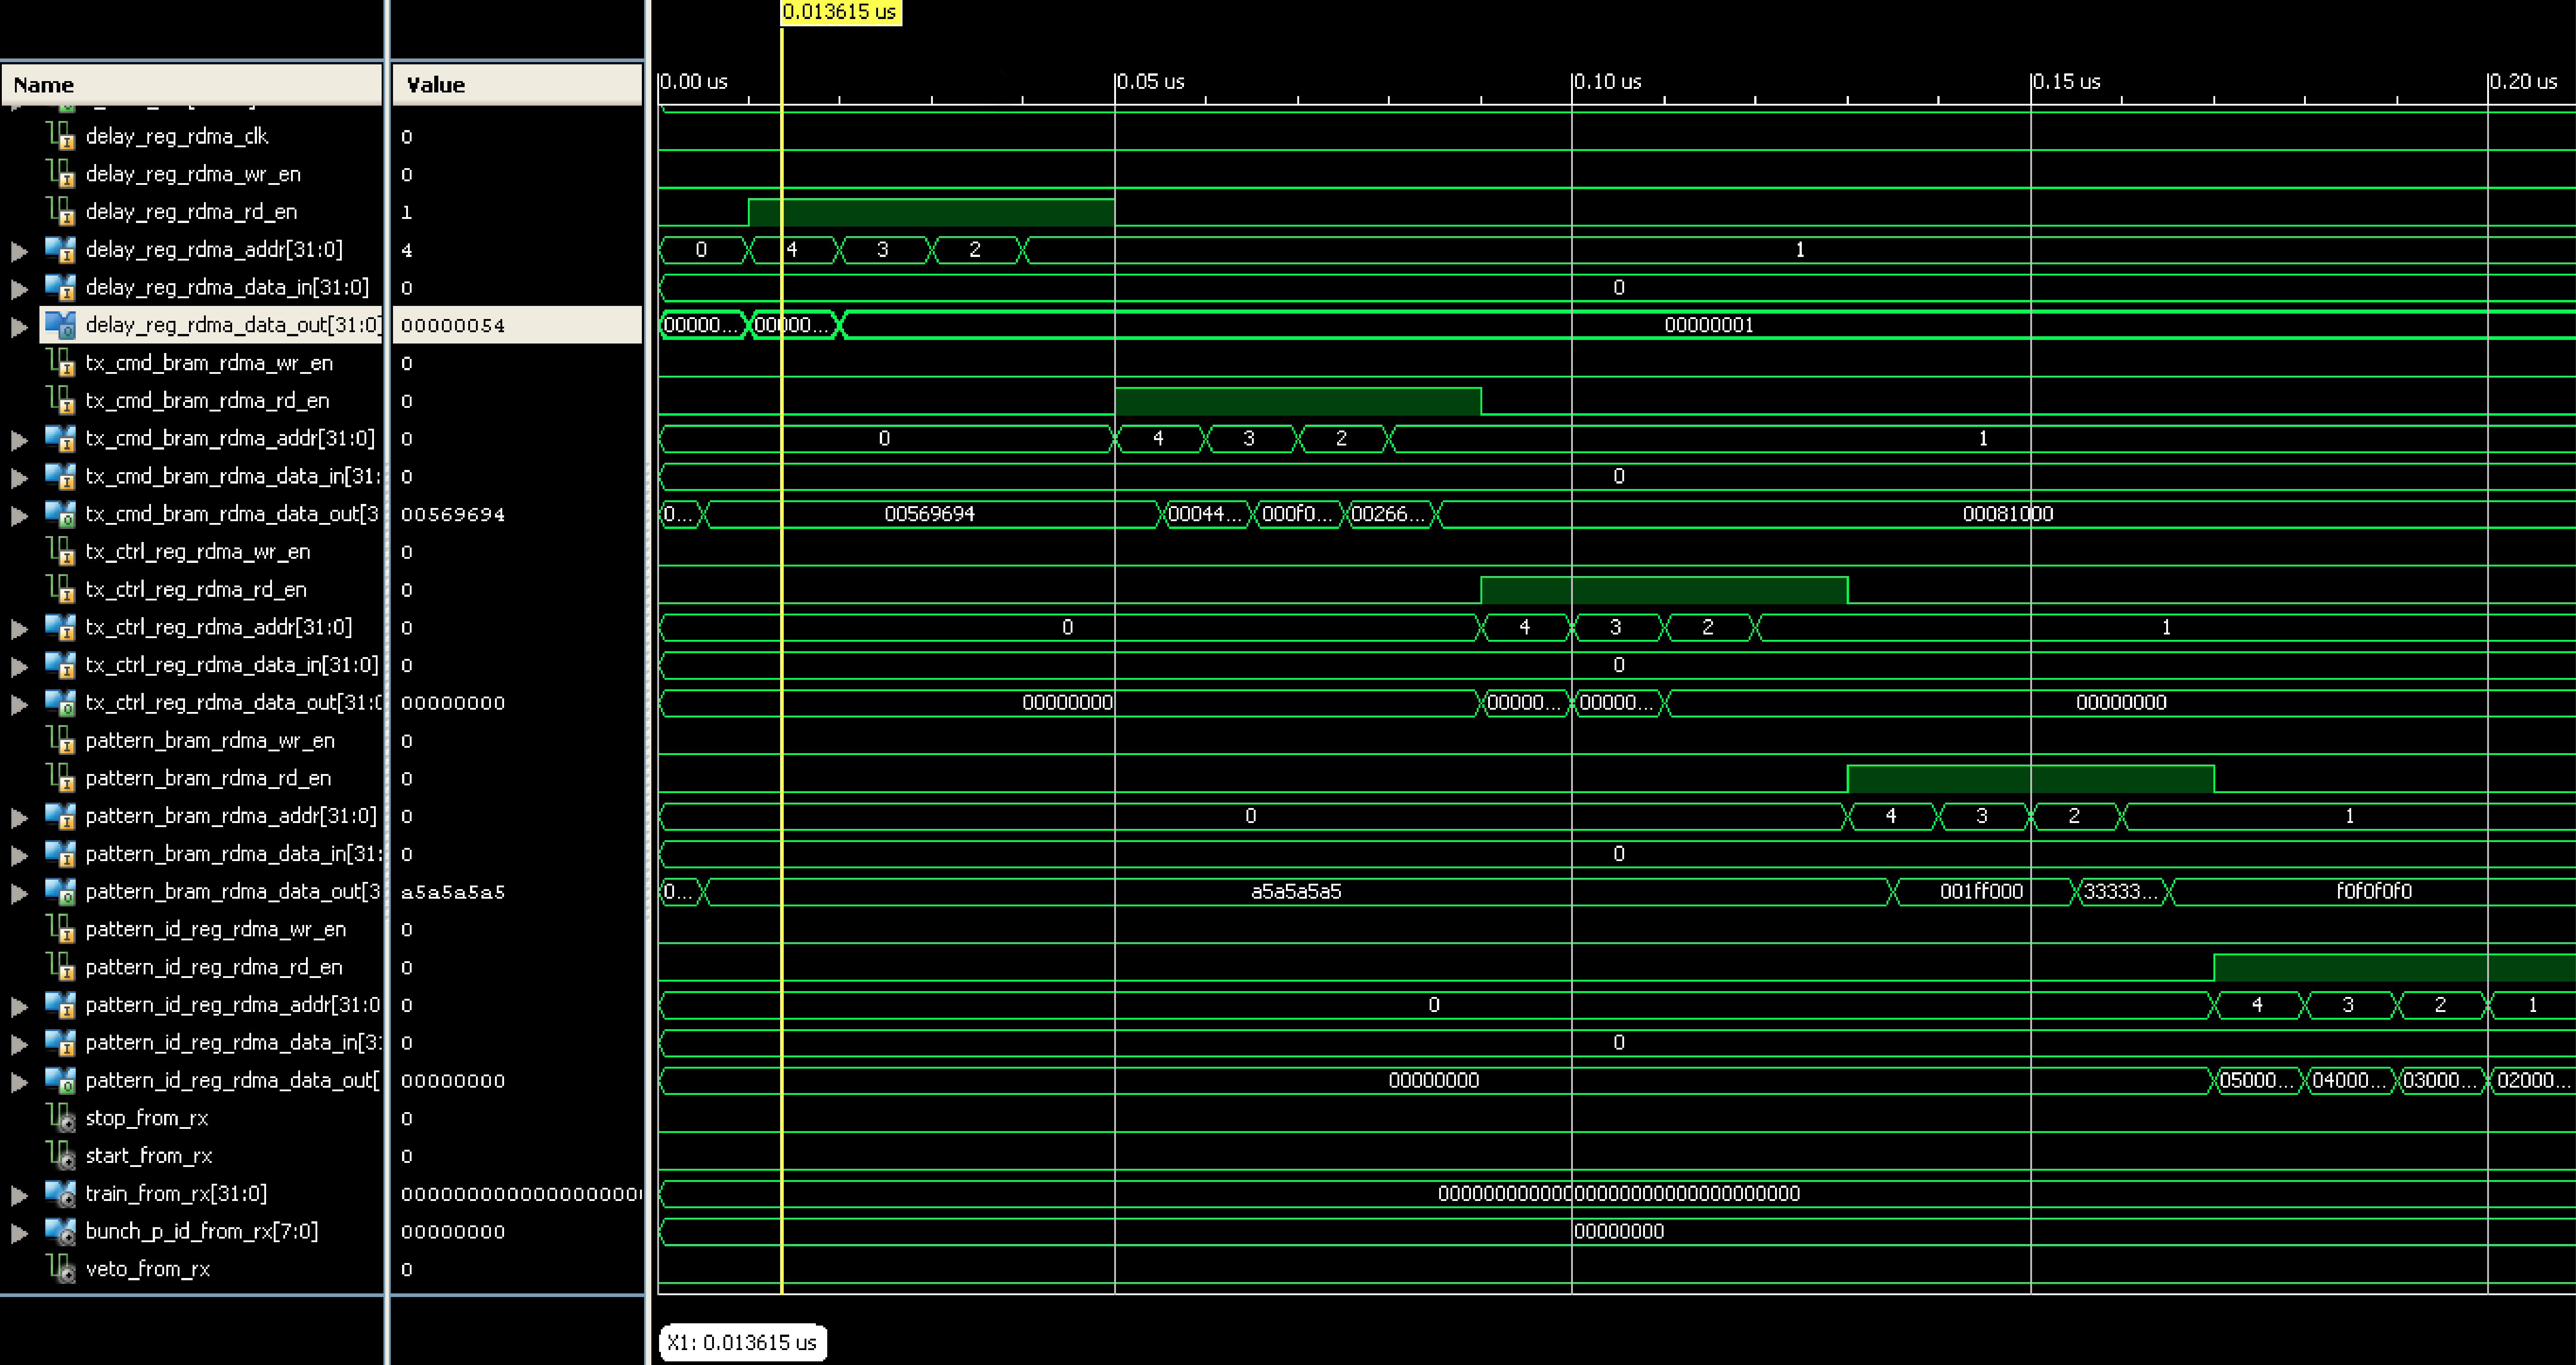
\includegraphics[width=\textwidth]{images/isim/edited/rdma.png}
        \caption{Read back of the first 4 locations of every block accessible via RDMA.}
        \label{fig:isim_rdma}
    \end{figure}
    
    % section rdma (end)
    \section{Local Link} % (fold)
    \label{sec:local_link}
    A sample read-out of the veto-log is shown in figure~\ref{fig:isim_locallink}.
    \begin{figure}[htbp]
        \centering
        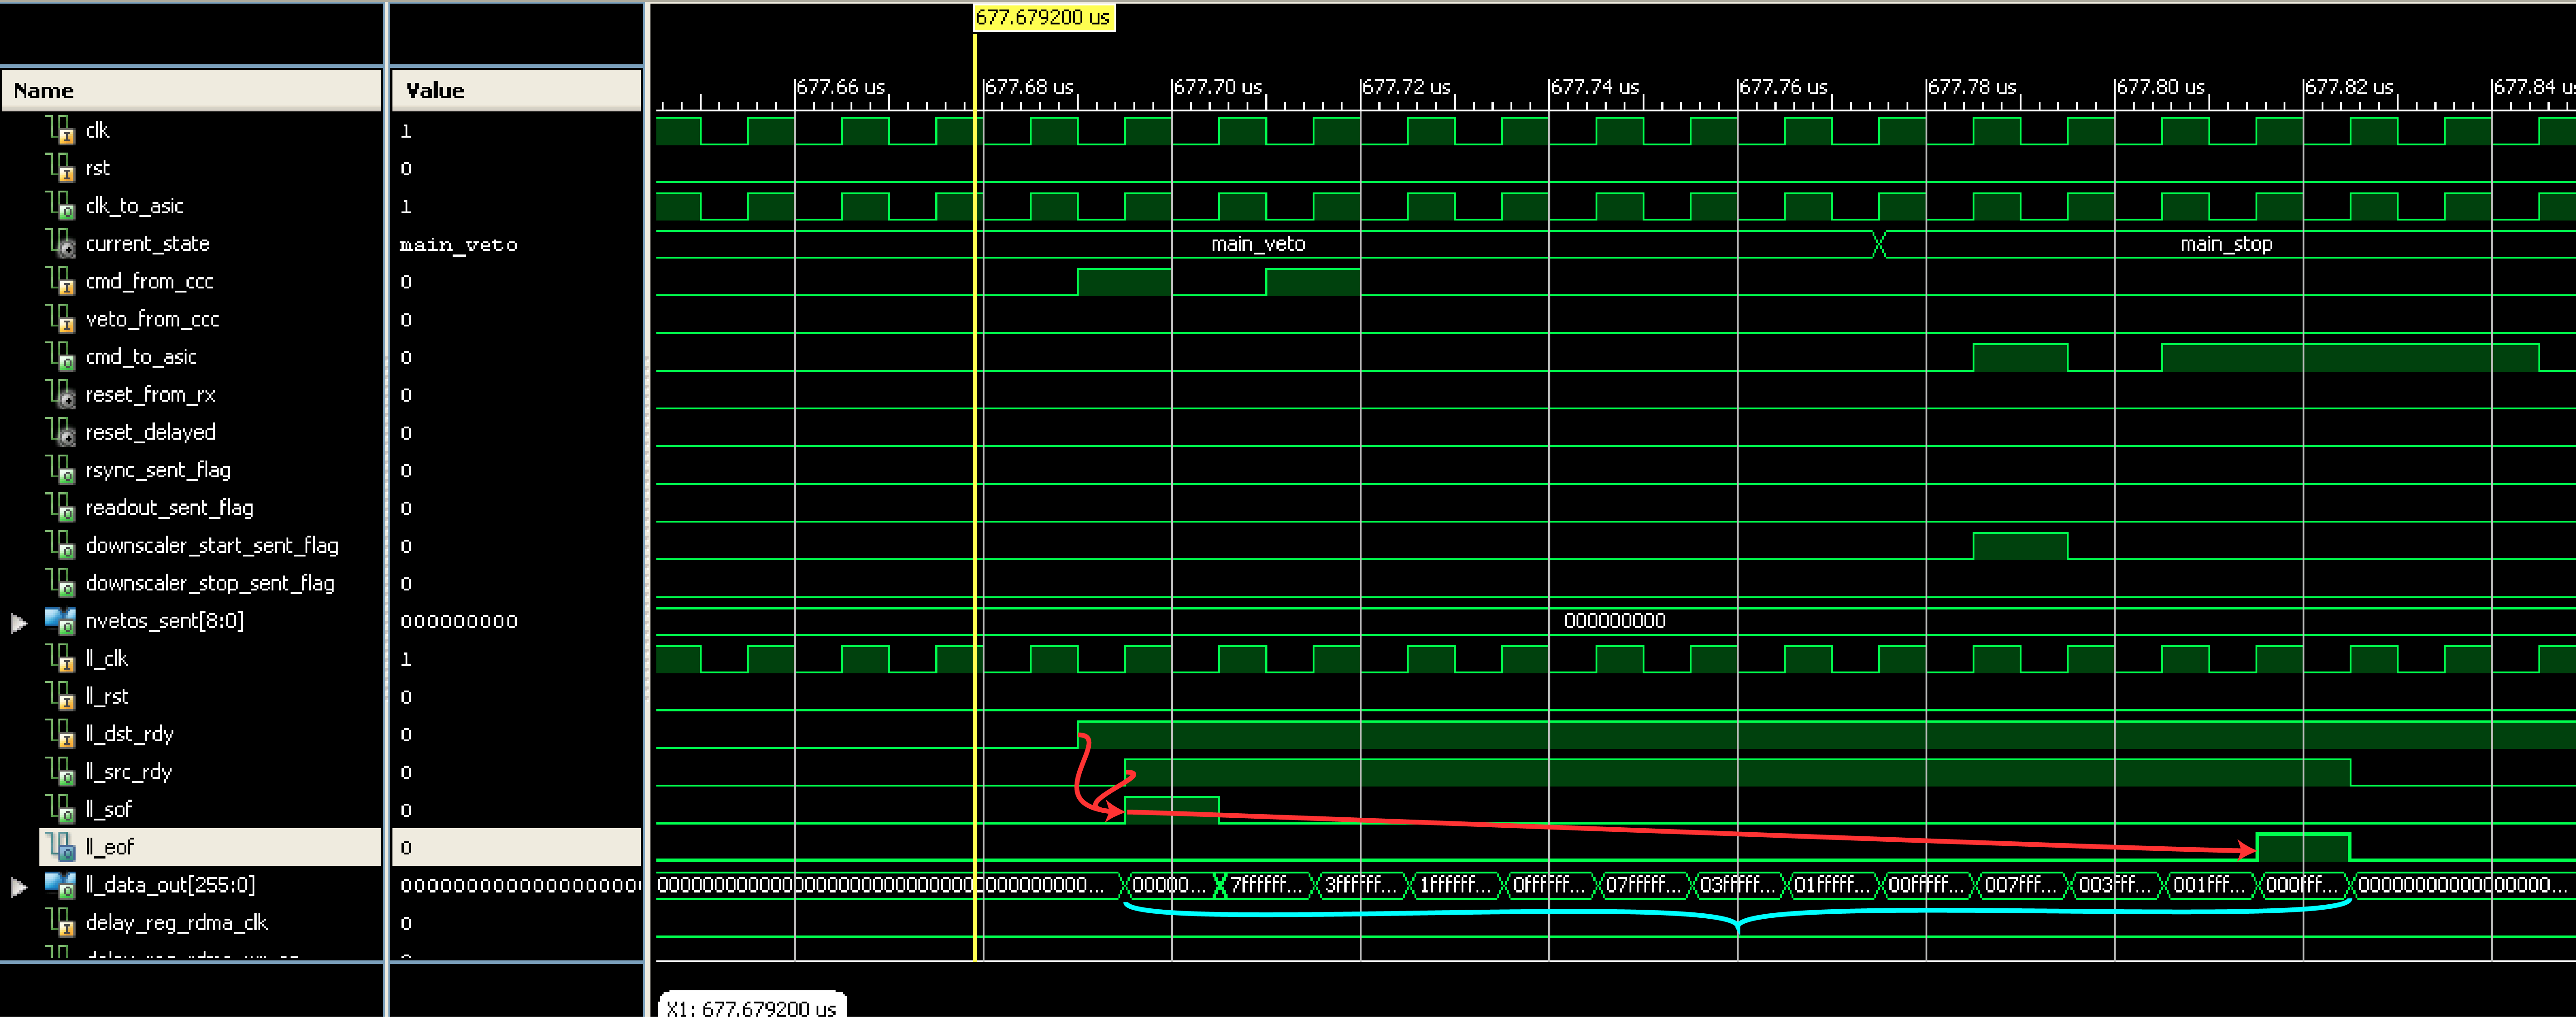
\includegraphics[width=\textwidth]{images/isim/edited/locallink.png}
        \caption{Read-out of the veto log for 3072 bunches.}
        \label{fig:isim_locallink}
    \end{figure}
    
    % section local_link (end)
    % chapter timing_diagrams (end)
    \appendix
    \chapter{ASIC command words} % (fold)
    \label{cha:asic_command_words}
    
    \begin{table}
        \begin{center}
            \setlength{\extrarowheight}{1.5pt}
            \begin{tabular}{c | l}
                Word & Name \\
                \hline  
                0x00 & NOP \\
                0x01 & STAND\_BY \\
                0x02 & POWER\_UP \\
                0x03 & ON\_CHIP\_RESET\_DISABLE \\
                0x04 & ON\_CHIP\_RESET\_ENABLE \\
                0x05 & RESET\_PRE\_AMP \\
                0x06 & RESET\_GAIN\_FRONT \\
                0x07 & RESET\_GAIN\_BACK \\
                0x08 & Reserved \\
                0x09 & TEST\_MODE\_D \\
                0x0A & TUNE\_MODE \\
                0x0B & CLEAR\_SKIP\_REGISTER \\
                0x0C & RESET\_WRITE\_POINTER \\
                0x0D & RESET\_TRIGGER\_POINTER \\
                0x0E & START\_WRITE\_POINTER \\
                0x0F & START\_TRIGGER\_POINTER \\
                0x10 & TRIGGER\_FLAG\_SET \\
                0x11 & READ\_OUT\_DATA \\
                0x12 & REMOVE\_RESET\_PRE\_AMP \\
                0x13 & REMOVE\_RESET\_GAIN\_STAGE1 \\
                0x14 & REMOVE\_RESET\_GAIN\_STAGE2 \\
                0x15 & CLOCK\_DIV\_SEL \\
                0x16 & SELF\_TEST\_EN \\
                0x17 & STOP\_READ\_OUT \\
                0x18 & RESET\_STATE\_MACHINE \\
                0x5A5A5 & SYNC\_RESET \\
            \end{tabular}
        \end{center}
        \caption{ASIC command words, see \cite{lpd_manual} for a full description and recommended use of these commands.}
        \label{tab:asic_command_words}
    \end{table}
    % section asic_command_words (end)
    %%%%%%%%%%%%%%%%%%%%%%%%%%%%%%%%%%%%%%%%%%%%%%%%%%%
    \chapter{RDMA interface} % (fold)
    \label{cha:rdma_interface}
    The RDMA interfaces used throughout the project have the interface seen in table~\ref{tab:rdma_interface}. The appropriate mask for the address is given in appropriate interface notes. In general for BRAMs a size of 32\(\times\)1024 the appropriate bits are 9:0 whilst for registers the bits 3:0 are used. 
    
    \begin{table}
        \begin{center}
            \begin{tabulary}{\textwidth}{l|c|c|L}
                Name & Direction & Type & Notes \\
                \hline
                clk       & \multirow{6}{*}{in}
                & std\_logic                & The RDMA clock (this can be separate from e.g. the CCC clock).\\
                rst       &     & std\_logic                & Reset the memory to some default state.                       \\
                rd\_en    &     & std\_logic                & Enable read operations at the address.                        \\
                wr\_en    &     & std\_logic                & Enable write operations at the address.                       \\
                addr      &     & std\_logic\_vector (31:0) & The address the MSB will be masked.                           \\
                data\_in  &     & std\_logic\_vector (31:0) & Used for writing and otherwise ignored.                       \\
                \hline
                data\_out & out & std\_logic\_vector (31:0) & Data out, only guaranteed for read operations.                \\
        
            \end{tabulary}
        \end{center}
        \caption{Standard RDMA interface.}
        \label{tab:rdma_interface}
    \end{table}
    % section rdma_interface (end)
    %%%%%%%%%%%%%%%%%%%%%%%%%%%%%%%%%%%%%%%%%%%%%%%%%%%
    \chapter{Local Link interface} % (fold)
    \label{cha:local_link_interface}
    The Local Link~\cite{locallink_spec} interface is used only to read out the veto log. The details of the frame composition are given in section~\ref{cha:veto_filter}. The interface used is minimal (i.e. no optional features are used) and given in table~\ref{tab:local_link_interface}.
    \begin{table}
        \begin{center}
            \begin{tabulary}{\textwidth}{l | c | c | L}
                Name & Direction & Type & Notes \\
                \hline
                clk        & \multirow{3}{*}{in} 
                & std\_logic                 & The LL clock (this can be separate from e.g. the CCC clock).\\
                rst        &     & std\_logic                 & Abort.                                                      \\
                dst\_rdy   &     & std\_logic                 & Destination ready.                                          \\
                \hline
                src\_rdy   & \multirow{4}{*}{out}
                & std\_logic                 & Source ready i.e. this block.                               \\
                sof        &     & std\_logic                 & Start of frame flag.                                        \\
                eof        &     & std\_logic                 & End of frame flag.                                          \\
                data\_out  &     & std\_logic\_vector (255:0) & Data out.                                                   \\
            \end{tabulary}
        \end{center}
        \caption{Minimal local link interface as used by the veto logger.}
        \label{tab:local_link_interface}
    \end{table}
  
    % section local_link_interface (end)
    %%%%%%%%%%%%%%%%%%%%%%%%%%%%%%%%%%%%%%%%%%%%%%%%%%%
    % \bibliographystyle{plain}
%     \bibliography{ral_manual}

\end{document}
    
